\documentclass[a4paper]{article}
\usepackage{minted}

\usepackage{polski}
\usepackage[utf8]{inputenc}

\usepackage[export]{adjustbox}
\usepackage{scrextend}
\usepackage{amsfonts}
\usepackage{amsmath}


\usepackage{geometry}
\geometry{a4paper, left=15mm, top=30mm, right=15mm, bottom=20mm}

\usepackage{gensymb}
\usepackage{graphicx} 
\usepackage{isotope}
\usepackage{array}
\usepackage{float}
\usepackage{titlesec}
\usepackage{fancyhdr}
\usepackage{multirow}

\usepackage{hyperref}
\usepackage{sectsty}
\usepackage{enumitem}
\usepackage{listings}
\usepackage[labelformat=simple]{subcaption}
\usepackage{xcolor,colortbl}


\usepackage{tikz}
\usetikzlibrary{shapes.geometric, arrows}
\tikzstyle{startstop} = [
    rectangle, 
    rounded corners, 
    minimum width=3cm, minimum height=1cm,
    text centered,
    draw=black, fill=red!30]
\tikzstyle{io} = [
    trapezium, trapezium left angle=70, trapezium right angle=110, 
    minimum width=3cm, minimum height=1cm, 
    text centered, 
    draw=black, fill=blue!30]
\tikzstyle{process} = [
    rectangle, 
    minimum width=3cm, minimum height=1cm, 
    text centered, 
    draw=black, fill=orange!30]
\tikzstyle{decision} = [
    diamond, 
    minimum width=3cm, minimum height=1cm, 
    text centered, 
    draw=black, fill=green!30]
\tikzstyle{arrow} = [thick,->,>=stealth]

\usepackage{karnaugh-map}

\sectionfont{\normalfont\huge\sectionrule{0pt}{0pt}{-6pt}{1pt}}
\subsectionfont{\normalfont\LARGE}
\subsubsectionfont{\normalfont\Large}

\pagestyle{fancy}
\fancyhf{}
\fancyhead[LE,LO]{\Large Łukasz Kwinta, Kacper Kozubowski, Ida Ciepiela}
\fancyhead[LE,RO]{\Large Sterownik windy}
\fancyfoot[CE,CO]{\Large\thepage}

\renewcommand{\footrulewidth}{1pt}
\renewcommand{\headrulewidth}{1pt}

\definecolor{Gray}{gray}{0.85}
\definecolor{LightGray}{gray}{0.95}

\newcolumntype{a}{>{\columncolor{Gray}}c}
\newcolumntype{b}{>{\columncolor{white}}c}

\hypersetup{
    colorlinks,
    citecolor=black,
    filecolor=black,
    linkcolor=black,
    urlcolor=black
}

\counterwithin{table}{section}
\counterwithin{figure}{section}

\title{\fontsize{30pt}{30pt}\selectfont Laboratorium 3 \\ Sterownik windy}
\author{\fontsize{20pt}{20pt}\selectfont Łukasz Kwinta, Kacper Kozubowski, Ida Ciepiela}
\date{maj 2024}

\begin{document}
\maketitle
\pagebreak
\large
\tableofcontents

\pagebreak
\section{Cel zadania}
\Large
Proszę zaproponować, zbudować i przetestować układ sterujący windą w przykładowym trzykondygnacyjnym budynku.

Winda posiada:
\begin{itemize}
    \item wskaźnik ruchu windy
    \item wskaźnik kierunku ruchu windy
    \item trzy czujniki otwarcia drzwi, po jednym na każdej kondygnacji
    \item trzy przyciski przywołania windy, po jednym na każdej kondygnacji
    \item trzy przyciski wyboru piętra w kabinie windy.
\end{itemize}

Winda powinna posiadać stale aktualizowany wskaźnik aktualnego piętra.

Rzeczy niedopowiedziane w treści zadania, proszę ustalić, doprecyzować i opisać samodzielnie.

\pagebreak
\section{Rozwiązanie}
Postanowiliśmy rozbić problem na wiele mniejszych problemów i rozwiązać je osobno aby 
na końcu połączyć je w jeden działający system. Poniżej zamieszczamy schemat 
przedstawiający połączenie poszczególnych układów, których działanie opiszemy szczegółowo poniżej.

\begin{figure}[H]
    \centering
    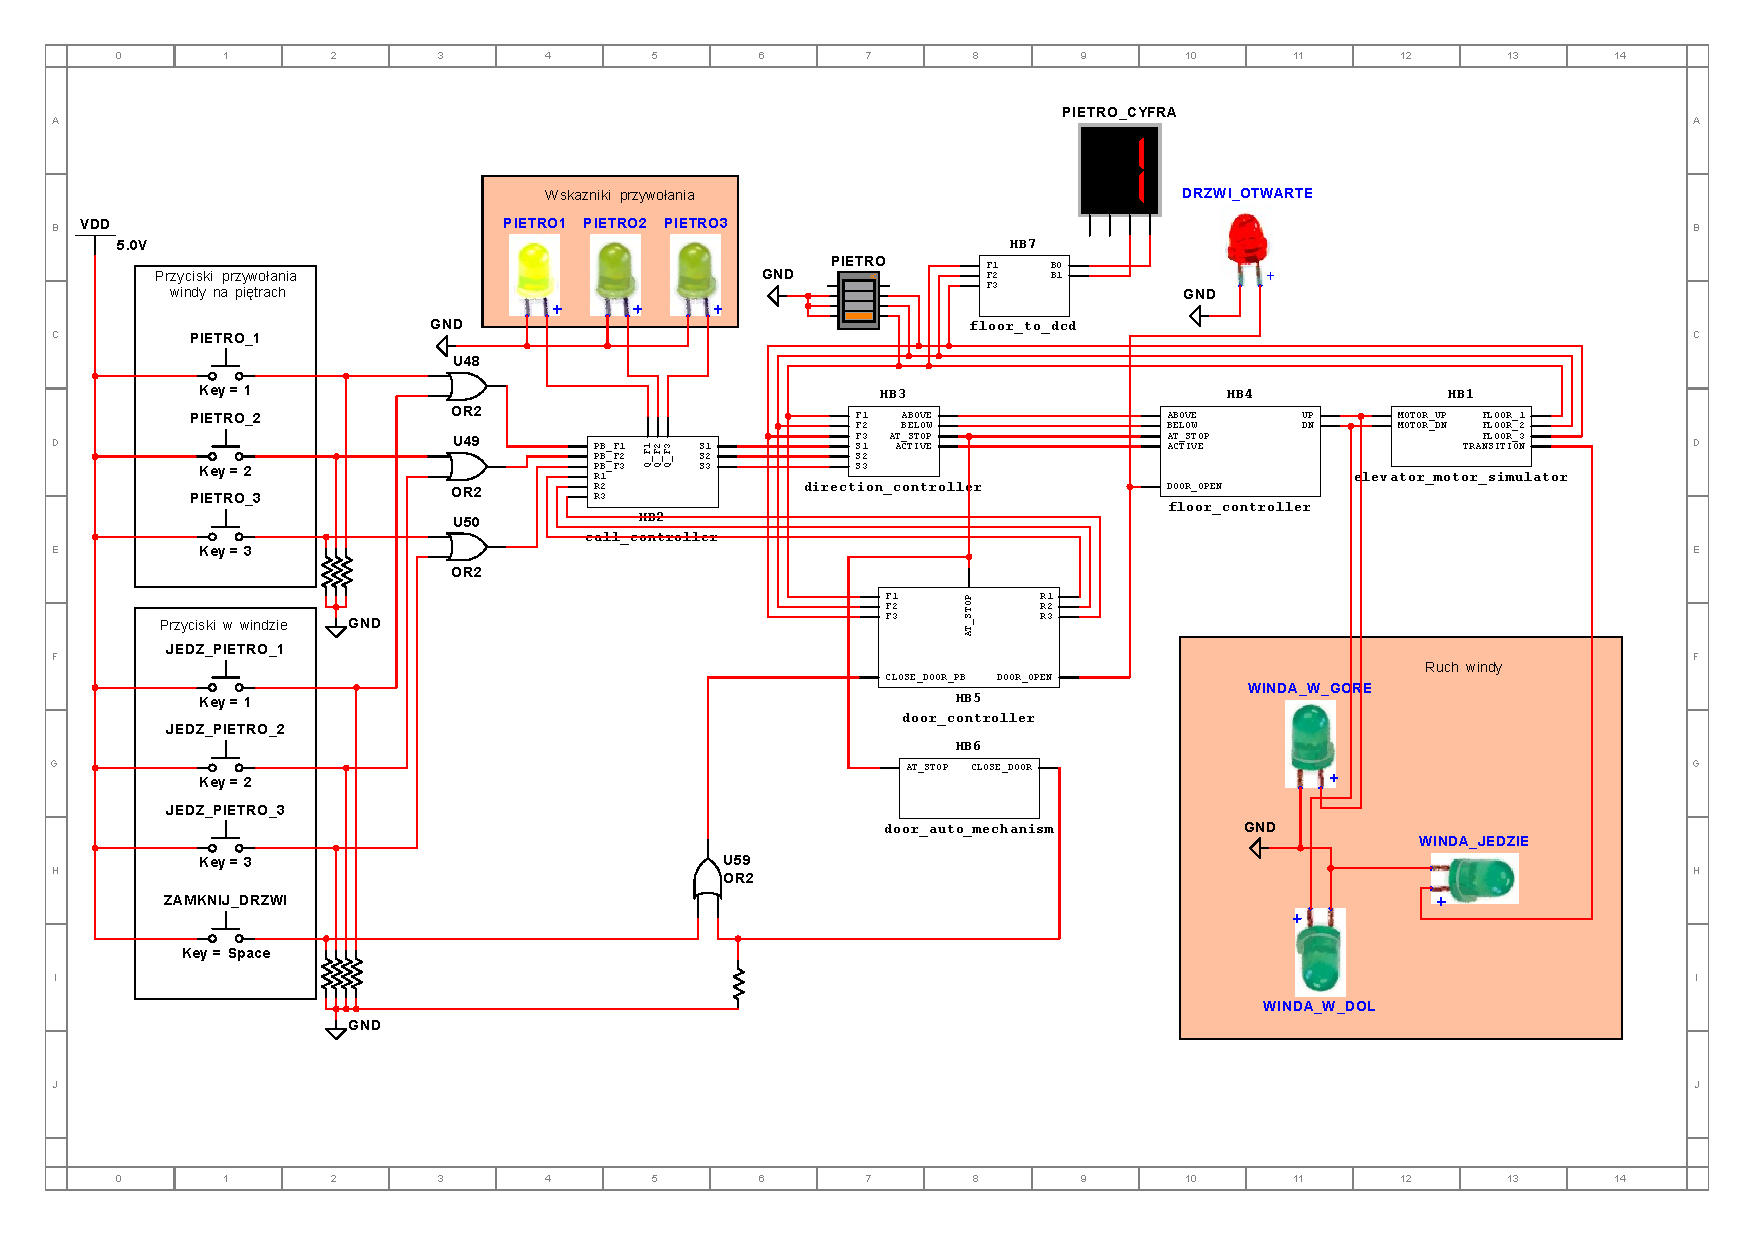
\includegraphics[width=\textwidth]{elevator_system_schemat.pdf}
    \caption{Schemat całego układu}
\end{figure}

\pagebreak
\subsection{Symulator silnika windy}
Aby zasymulować ruch windy wraz z czasem przemieszczania się między piętrami, zdecydowaliśmy się 
zaimplementować układ bazujący na liczniku i demultiplexerze.

\subsubsection{Black box}
Poniżej zamieszczamy schemat wyjść i wejść oraz opis logiki układu.
\begin{figure}[H]
    \centering
    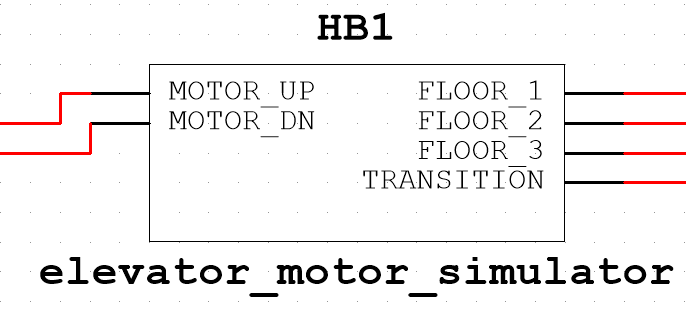
\includegraphics[width=0.6\textwidth]{elevator_motor_simulator.png}
    \caption{Black box układu symulującego silnik windy}
\end{figure}
\subsubsection{Wejścia}
\begin{itemize}
    \item \verb|MOTOR_UP| - sygnał wejściowy nakazujący poruszać się windzie w górę
    \item \verb|MOTOR_DN| - sygnał wejściowy nakazujący poruszać się windzie w dół
\end{itemize}
\subsubsection{Wyjścia}
\begin{itemize}
    \item \verb|FLOOR_1| - sygnał wyjściowy informujący o tym, że winda znajduje się na 1 piętrze,
                            aktywny w stanie wysokim
    \item \verb|FLOOR_2| - sygnał wyjściowy informujący o tym, że winda znajduje się na 2 piętrze,
                            aktywny w stanie wysokim
    \item \verb|FLOOR_3| - sygnał wyjściowy informujący o tym, że winda znajduje się na 3 piętrze,
                            aktywny w stanie wysokim
    \item \verb|TRANSITION| - sygnał wyjściowy informujący o tym że winda jest obecnie w ruchu,
                            aktywny w stanie wysokim
\end{itemize}
\subsubsection{Realizacja układu}
Do realizacji układu wykorzystaliśmy 4 bitowy licznik z biblioteki komponentów programu Multisim,
układ \verb|74LS193N|. Poniżej zamieszczamy tabelkę przedstawiającą działanie licznika:
\begin{center}
    \begin{tabular}{|c|c|c|c||c|}
        \hline \verb|CLR| & \verb|~LOAD| & \verb|Up| & \verb|Down| & Mode \\
        \hline H & X & X & X & Reset(Async.) \\
        \hline L & L & X & X & Preset(Async.) \\
        \hline L & H & H & H & No Change \\
        \hline L & H & $\uparrow$ & H & Count Up \\
        \hline L & H & H & $\uparrow$ & Count Down \\
        \hline
    \end{tabular}
    \captionof{table}{Źródło: \url{https://www.multisim.com/help/components/binary-counters/}}
\end{center}

\begin{abstract}
    \noindent \begin{itemize}
        \item H - stan wysoki na wejściu
        \item L - stan niski na wejściu
        \item X - dowolny stan na wejściu
        \item $\uparrow$ - narastające zbocze sygnału
    \end{itemize}
\end{abstract}
Stworzyliśmy układ kombinacyjny, który mapuje wyjście zegara, na adres demultiplexera, który 
z kolei przekazuje jedynkę logiczną na odpowiednie wyjście. 
Przyjęliśmy, że:
\begin{itemize}
    \item 0000 - winda jest na 1 piętrze
    \item 1000 - winda jest na 2 piętrze
    \item 1111 - winda jest na 3 piętrze
    \item każdy inny - winda porusza się między piętrami
\end{itemize}
Jako demultiplexer wykorzystaliśmy układ \verb|U7A 4555BD_5V|. Jest to demultiplexer 1: 4, z 2 
bitami adresowymi.

Do wyprowadzenia formuł wykorzystaliśmy skrypt w języku Python, który generuje tabelę prawdy oraz
minimalizuje formuły logiczne. Poniżej zamieszczamy kod programu oraz wynik jego działania:
\begin{minted}[
    frame=lines,
    framesep=2mm,
    baselinestretch=1.2,
    bgcolor=LightGray,
    fontsize=\footnotesize,
    linenos
]{python}
import logicmin
elevator_motor_mux_tt = logicmin.TT(4, 2)

for i in range(16):
    permutation = bin(i).removeprefix("0b").rjust(4, '0')
    
    a1 = '1'
    b1 = '1'

    if i == 0:
        a1 = '0'
        b1 = '0'
    elif i == 8:
        a1 = '1'
        b1 = '0'
    elif i == 15:
        a1 = '0'
        b1 = '1'

    elevator_motor_mux_tt.add(permutation, [a1, b1])

print("--------------------------------elevator_motor_tt")
sols = elevator_motor_mux_tt.solve()
print(sols.printN(xnames=['QD', 'QC', 'QB', 'QA'],ynames=['1A', '1B']))
\end{minted}
Wynikiem działania skryptu są zminimalizowane formuły logiczne:

\begin{verbatim}
--------------------------------elevator_motor_tt
1B <= QA + QB + QC
1A <= QD'.QA + QC'.QB + QC.QA' + QD.QB'
\end{verbatim}

Po zaimplementowaniu układu w programie Multisim, uzyskaliśmy następujący schemat:
\begin{figure}[H]
    \centering
    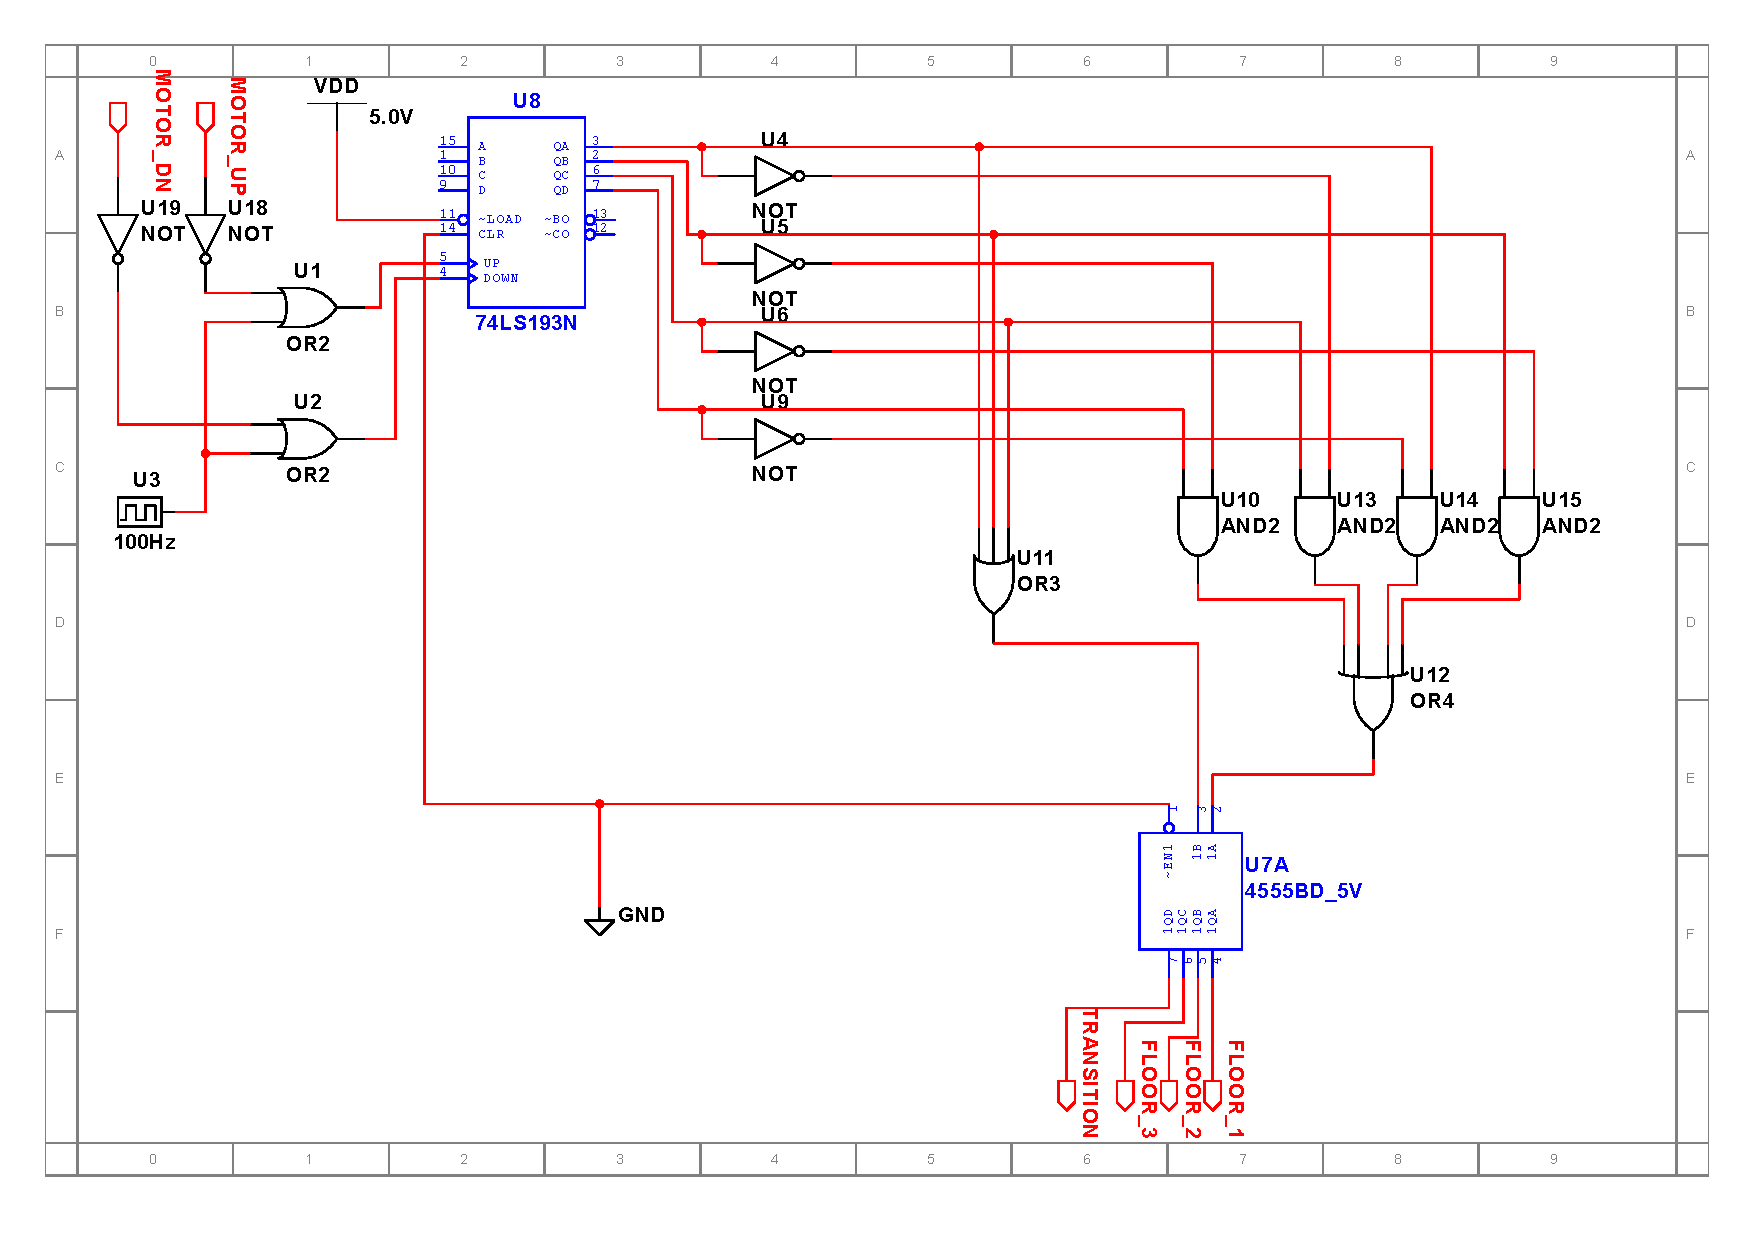
\includegraphics[width=\textwidth]{elevator_motor_simulator_schemat.pdf}
    \caption{Schemat układu symulującego silnik windy}
\end{figure}

Bramki logiczne \verb|NOT| i \verb|OR| na wejściu układu służą do przekazywania stanu wysokiego 
lub zegara na wejście licznika. Zgodnie z tabelką działania licznika zapewniają one, że 
w momencie gdy chcemy liczyć do góry, układ przekazuje stan wysoki na wejście licznika \verb|DOWN|
oraz sygnał zegara na wejście licznika \verb|UP|.

\pagebreak

\subsection{Kontroler ruchu windy}

Prosty układ kombinacyjny przekazujący silnikowi sygnał o ruchu w danym kierunku gdy wszystkie warunki
na ruszenie windą zostaną spełnione.

\subsubsection{Black box}
\begin{figure}[H]
    \centering
    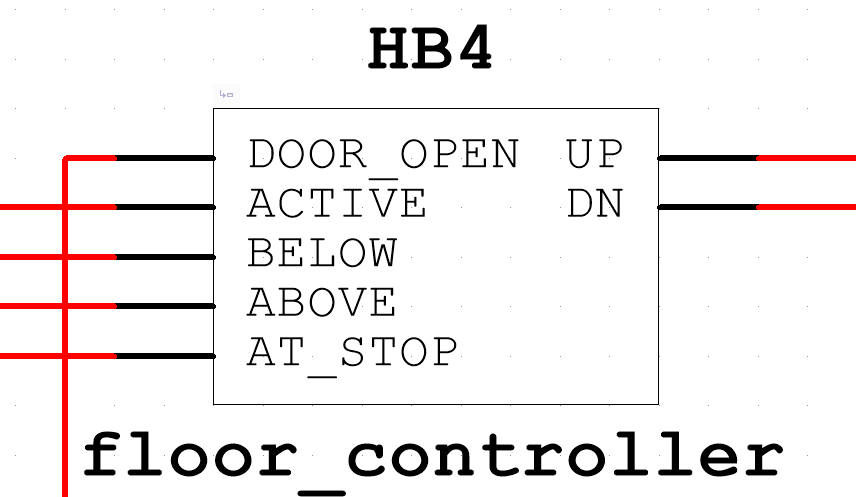
\includegraphics[width=0.6\textwidth]{floor_controller.png}
    \caption{Black box układu inicjującego ruch windy}
\end{figure}

\subsubsection{Wejścia}
\begin{itemize}
    \item \verb|DOOR_OPEN| - sygnał wejściowy informujący o stanie otwarcia drzwi
    \item \verb|ACTIVE| - sygnał wejściowy informujący, że winda otrzymała wezwanie
    \item \verb|BELOW| - sygnał wejściowy informujący, że piętro docelowe znajduje się poniżej obecnej pozycji windy
    \item \verb|ABOVE| - sygnał wejściowy informujący, że piętro docelowe znajduje się powyżej obecnej pozycji windy
    \item \verb|AT_STOP| - sygnał wejściowy informując, że winda znajduje się na piętrze na, które została wezwana
\end{itemize}

\subsubsection{Wyjścia}
\begin{itemize}
    \item \verb|UP| - sygnał wyjściowy informujący o gotowości do ruchu w górę
    \item \verb|DN| - sygnał wyjściowy informujący o gotowości do ruchu w dół
\end{itemize}

\subsubsection{Realizacja układu}
W realizacji układu wykorzystaliśmy dwa przerzutniki SR, które są ustawiane w momencie gdy wszystkie
warunki do ruchu w danym kierunku są spełnione i resetowane gdy spełnione są wszystkie warunki konieczne
do zatrzymania windy.

Poniżej przedstawiony został kod programu w języku Python, który wykorzystaliśmy do wyprowadzenia
formuł logicznych.
\begin{minted}[
    frame=lines,
    framesep=2mm,
    baselinestretch=1.2,
    bgcolor=LightGray,
    fontsize=\footnotesize,
    linenos
]{python}
import logicmin
floor_controller_tt = logicmin.TT(5, 4)

for i in range(32):
    permutation = bin(i).removeprefix("0b").rjust(5, '0')
    
    variables = {
        'DOOR_OPEN': int(permutation[0]),
        'ACTIVE': int(permutation[1]),
        'BELOW': int(permutation[2]),
        'ABOVE': int(permutation[3]),
        'AT_STOP': int(permutation[4])
    }

    set_up = '0'
    reset_up = '0'
    set_dn = '0'
    reset_dn = '0'

    if not variables['ABOVE'] and not variables['BELOW'] and variables['AT_STOP']:
        set_up = '0'
        reset_up = '1'
        set_dn = '0'
        reset_dn = '1'

    elif variables['ACTIVE'] and variables['BELOW'] and not variables['DOOR_OPEN']:
        set_up = '0'
        reset_up = '0'
        set_dn = '1'
        reset_dn = '0'

    elif variables['ACTIVE'] and variables['ABOVE'] and not variables['DOOR_OPEN']:
        set_up = '1'
        reset_up = '0'
        set_dn = '0'
        reset_dn = '0'

    floor_controller_tt.add(permutation, [set_up, reset_up, set_dn, reset_dn])

print("--------------------------------floor_controller_tt")
sols = floor_controller_tt.solve()
print(sols.printN(xnames=['DOOR_OPEN', 'ACTIVE', 'BELOW', 'ABOVE', 'AT_STOP'],
                ynames=['SET_UP', 'RESET_UP','SET_DN', 'RESET_DN']))
\end{minted}

\pagebreak
Wynikiem działania skryptu są zminimalizowane formuły logiczne:

\begin{verbatim}
--------------------------------floor_controller_tt
RESET_DN <= BELOW'.ABOVE'.AT_STOP
SET_DN <= DOOR_OPEN'.ACTIVE.BELOW
RESET_UP <= BELOW'.ABOVE'.AT_STOP
SET_UP <= DOOR_OPEN'.ACTIVE.BELOW'.ABOVE
\end{verbatim}

Na podstawie otrzymanych formuł zaimplementowaliśmy w programie Multisim,
niżej przedstawiony schemat.

\begin{figure}[H]
    \centering
    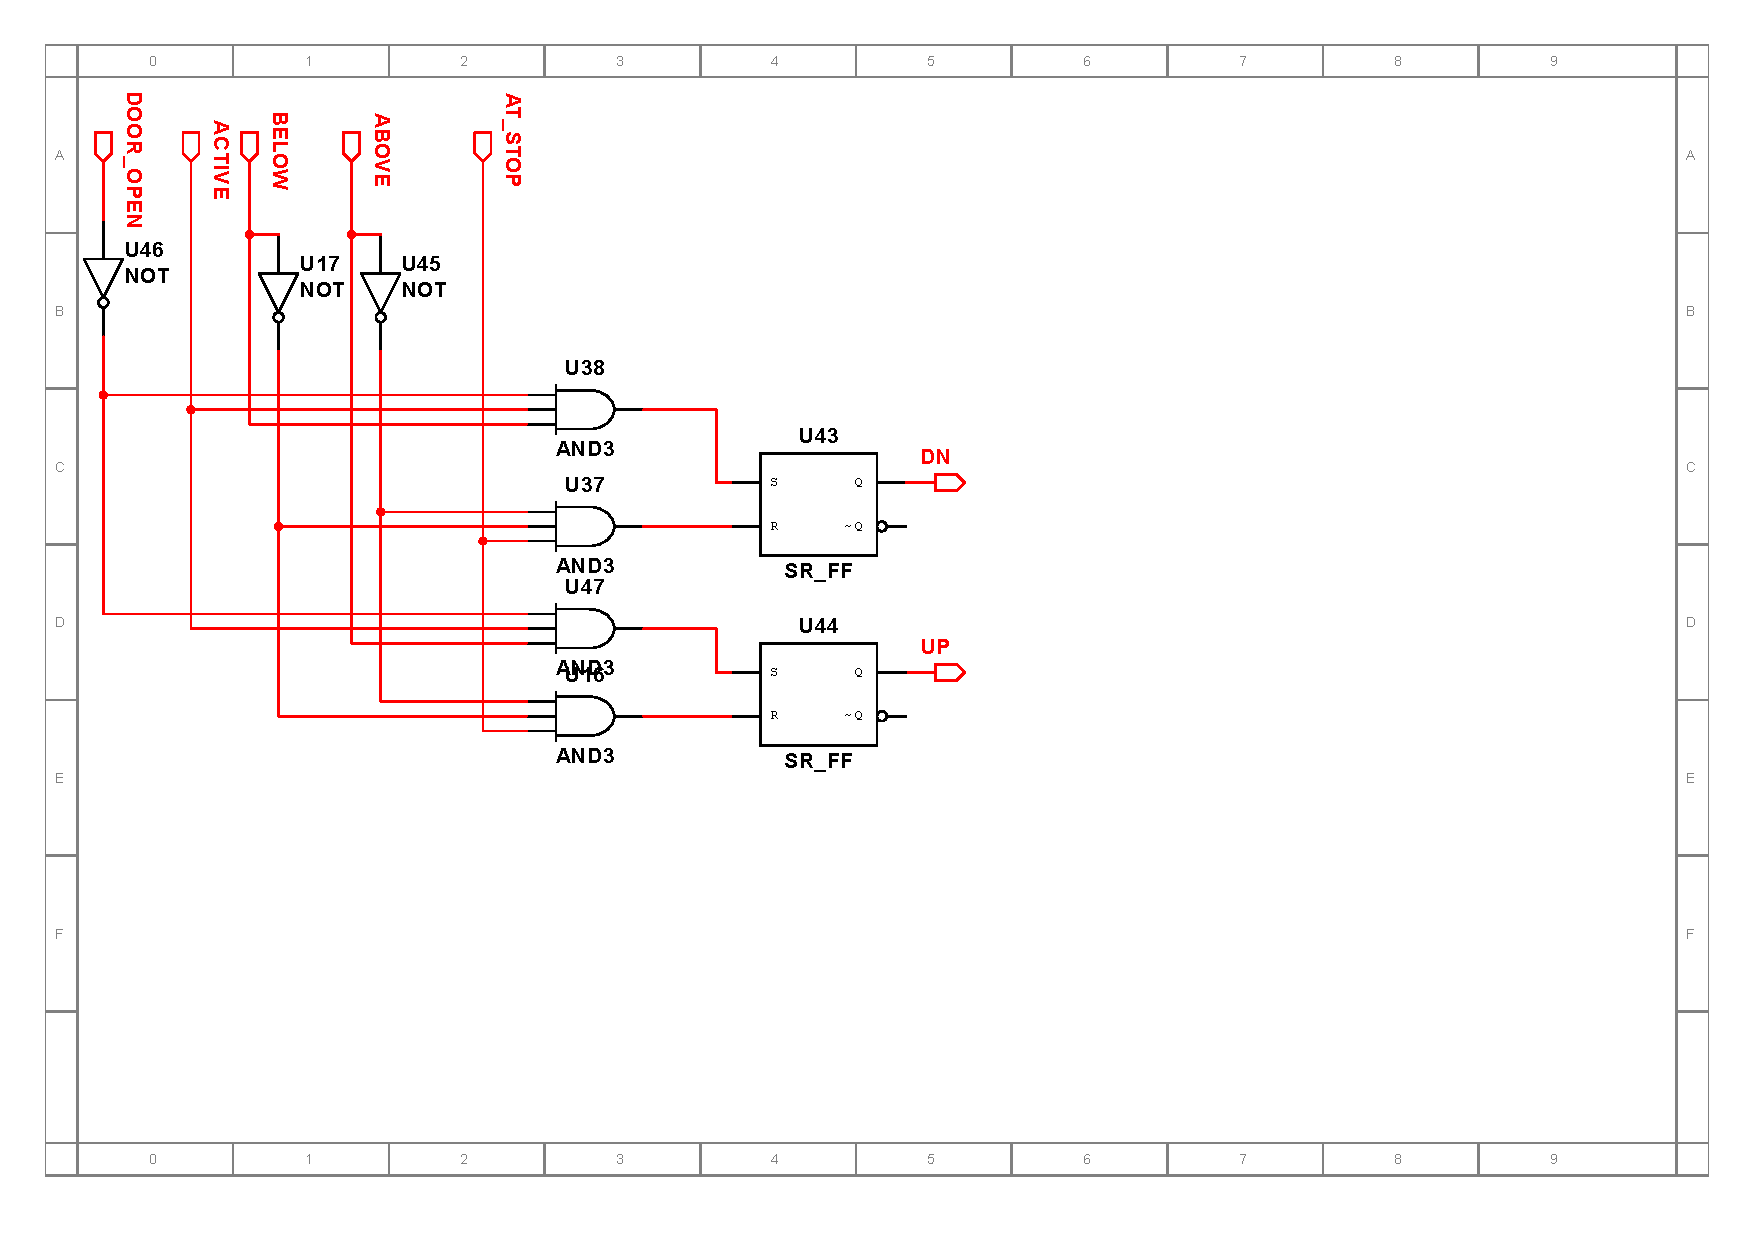
\includegraphics[width=\textwidth]{floor_controller_schemat.pdf}
    \caption{Schemat układu inicjującego ruch windy}
\end{figure}

\pagebreak
\subsection{Kontroler kierunku ruchu}

Układ, który na podstawie otrzymanego wezwania rozpoznaje względną pozycję piętra docelowego
w odniesieniu do obecnego położenia windy.

\subsubsection{Black box}
\begin{figure}[H]
    \centering
    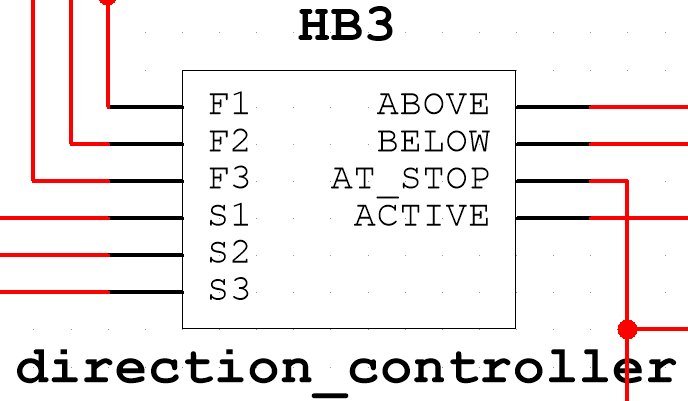
\includegraphics[width=0.6\textwidth]{direction_controller.png}
    \caption{Black box układu przetwarzającego wezwanie}
\end{figure}

\subsubsection{Wejścia}
\begin{itemize}
    \item \verb|F1| - sygnał wejściowy informujący o tym, że winda znajduje się na 1. piętrze
    \item \verb|F2| - sygnał wejściowy informujący o tym, że winda znajduje się na 2. piętrze
    \item \verb|F3| - sygnał wejściowy informujący o tym, że winda znajduje się na 3. piętrze
    \item \verb|S1| - sygnał wejściowy informujący o wezwaniu windy na 1. piętro
    \item \verb|S2| - sygnał wejściowy informujący o wezwaniu windy na 2. piętro
    \item \verb|S3| - sygnał wejściowy informujący o wezwaniu windy na 3. piętro
\end{itemize}

\subsubsection{Wyjścia}
\begin{itemize}
    \item \verb|ABOVE| - sygnał wyjściowy informujący, że piętro docelowe znajduje się powyżej obecnej pozycji windy  
    \item \verb|BELOW| - sygnał wyjściowy informujący, że piętro docelowe znajduje się poniżej obecnej pozycji windy
    \item \verb|AT_STOP| - sygnał wyjściowy informujący, że winda znajduje się na piętrze docelowym
    \item \verb|ACTIVE| - sygnał wyjściowy przekazujący dalej informację o otrzymaniu wezwania
\end{itemize}

\subsubsection{Realizacja układu}

Poniżej przedstawiony został kod programu w języku Python, który wykorzystaliśmy do wyprowadzenia
formuł logicznych.
\begin{minted}[
    frame=lines,
    framesep=2mm,
    baselinestretch=1.2,
    bgcolor=LightGray,
    fontsize=\footnotesize,
    linenos
]{python}
import logicmin
direction_controller_tt = logicmin.TT(6, 4)

for i in range(64):
    permutation = bin(i).removeprefix("0b").rjust(6, '0')
    
    variables = {
        'F1': int(permutation[0]),
        'F2': int(permutation[1]),
        'F3': int(permutation[2]),
        'S1': int(permutation[3]),
        'S2': int(permutation[4]),
        'S3': int(permutation[5])
    }

    above = '0'
    below = '0'
    at_stop = '0'
    active = '0'

    if variables['F1'] and (variables['S2'] or variables['S3']):
        above = '1'
    
    elif variables['F2'] and variables['S1']:
        below = '1'

    elif variables['F2'] and variables['S3']:
        above = '1'
    
    elif variables['F3']and (variables['S1'] or variables['S2']):
        below = '1'

    if (variables['F1'] and variables['S1']) or (variables['F2'] and variables['S2']) 
                    or (variables['F3'] and variables['S3']):
        at_stop = '1'

    if variables['S1'] or variables['S2'] or variables['S3']:
        active = '1'

    direction_controller_tt.add(permutation, [above, below, at_stop, active])

print("--------------------------------direction_controller_tt")
sols = direction_controller_tt.solve()
print(sols.printN(xnames=['F1', 'F2', 'F3', 'S1', 'S2', 'S3'],ynames=['ABOVE','BELOW', 'AT_STOP', 'ACTIVE']))
\end{minted}

\pagebreak
Wynikiem działania skryptu są zminimalizowane formuły logiczne:

\begin{verbatim}
--------------------------------direction_controller_tt
ACTIVE <= S3 + S2 + S1
AT_STOP <= F3.S3 + F2.S2 + F1.S1
BELOW <= F1'.F2'.F3.S2 + F1'.F3.S2.S3' + F3.S1.S2'.S3' + F2.S1.S2'.S3' + 
+ F1'.F3.S1 + F1'.F2.S1
ABOVE <= F2.S1'.S3 + F1.S3 + F1.S2
\end{verbatim}

Na podstawie otrzymanych formuł zaimplementowaliśmy w programie Multisim,
niżej przedstawiony schemat.

\begin{figure}[H]
    \centering
    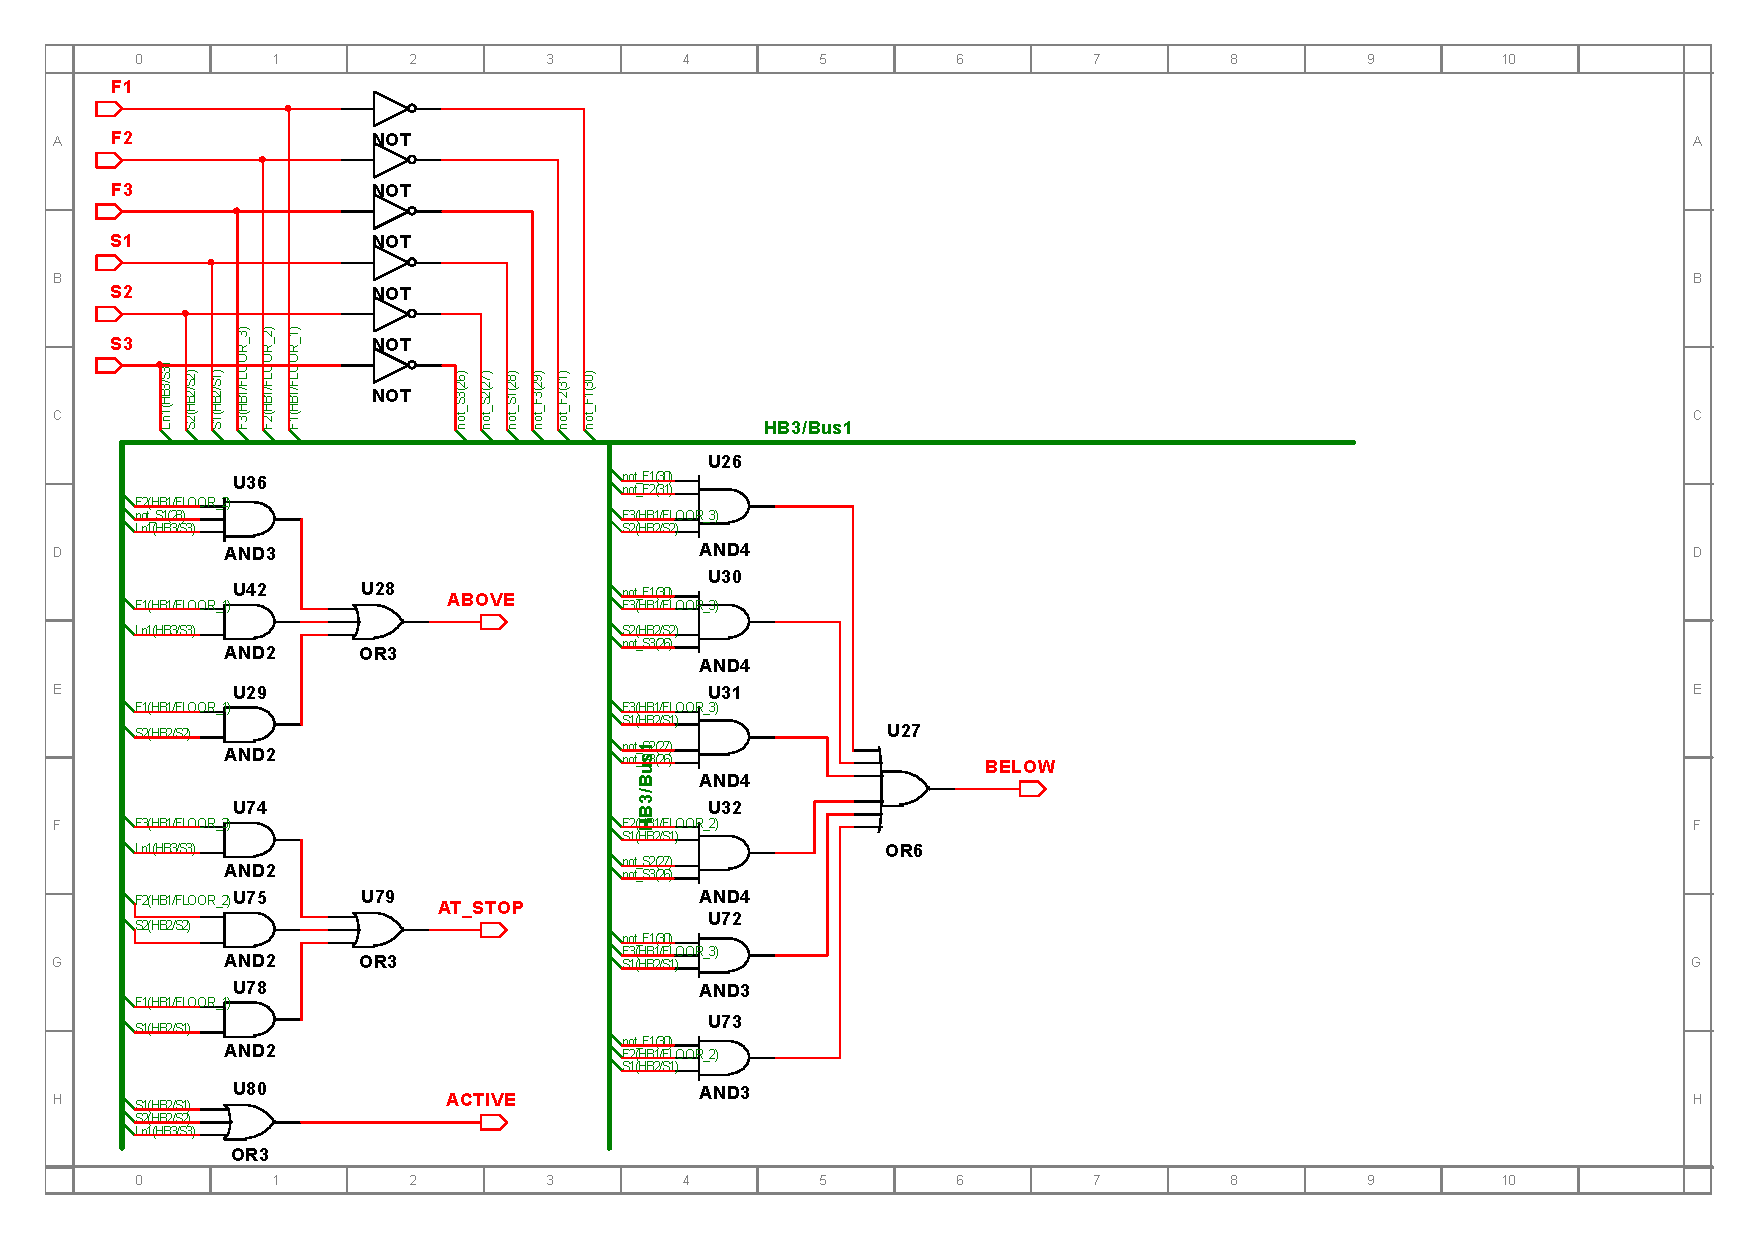
\includegraphics[width=\textwidth]{direction_controller_schemat.pdf}
    \caption{Schemat układu przetwarzającego wezwanie}
\end{figure}

\pagebreak
\subsection{Kontroler drzwi windy}

Układ zajmujący się obsługą drzwi po znalezieniu się windy na piętrze docelowym. 
Przetwarza on również informację o wykonaniu obsługiwanego wezwania
i wysyła sygnał do jego resetu.

\subsubsection{Black box}
\begin{figure}[H]
    \centering
    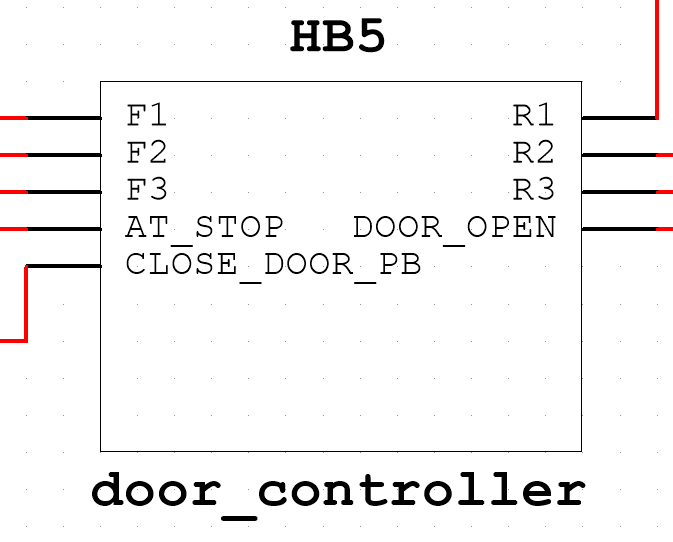
\includegraphics[width=0.6\textwidth]{door_controller.png}
    \caption{Black box układu kontrolującego obsługę drzwi}
\end{figure}

\subsubsection{Wejścia}
\begin{itemize}
    \item \verb|F1| - sygnał wejściowy informujący o tym, że winda znajduje się na 1. piętrze 
    \item \verb|F2| - sygnał wejściowy informujący o tym, że winda znajduje się na 2. piętrze
    \item \verb|F3| - sygnał wejściowy informujący o tym, że winda znajduje się na 3. piętrze
    \item \verb|AT_STOP| - sygnał wejściowy informujący, że winda znajduje się na piętrze docelowym
    \item \verb|CLOSE_DOOR_PB| - sygnał wejściowy nakazujący zamknięcie drzwi
\end{itemize}

\subsubsection{Wyjścia}
\begin{itemize}
    \item \verb|R1| - sygnał wyjściowy, informujący o wykonaniu wezwania na 1. piętro
    \item \verb|R2| - sygnał wyjściowy, informujący o wykonaniu wezwania na 2. piętro
    \item \verb|R3| - sygnał wyjściowy, informujący o wykonaniu wezwania na 3. piętro
    \item \verb|DOOR_OPEN| - sygnał wyjściowy, informujący o otwarciu drzwi
\end{itemize}

\subsubsection{Realizacja układu}

Poniżej przedstawiony został kod programu w języku Python, który wykorzystaliśmy do wyprowadzenia
formuł logicznych.
\begin{minted}[
    frame=lines,
    framesep=2mm,
    baselinestretch=1.2,
    bgcolor=LightGray,
    fontsize=\footnotesize,
    linenos
]{python}
import logicmin
door_controller_tt = logicmin.TT(5, 4)

for i in range(32):
    permutation = bin(i).removeprefix("0b").rjust(5, '0')
    
    variables = {
        'CLOSE_DOOR_PB': int(permutation[0]),
        'AT_STOP': int(permutation[1]),
        'F1': int(permutation[2]),
        'F2': int(permutation[3]),
        'F3': int(permutation[4])
    }

    r1 = '0'
    r2 = '0'
    r3 = '0'
    door_open = '0'

    if variables['AT_STOP']: door_open = '1'
    if variables['AT_STOP'] and variables['CLOSE_DOOR_PB']:
        if variables['F1']: r1 = '1'
        if variables['F2']: r2 = '1'
        if variables['F3']: r3 = '1'

    door_controller_tt.add(permutation, [r1, r2, r3, door_open])

print("--------------------------------door_controller_tt")
sols = door_controller_tt.solve()
print(sols.printN(xnames=['CLOSE_DOOR_PB', 'AT_STOP', 'F1', 'F2', 'F3'],ynames=['R1','R2', 'R3', 'DOOR_OPEN']))
\end{minted}
Wynikiem działania skryptu są zminimalizowane formuły logiczne:

\begin{verbatim}
--------------------------------door_controller_tt
DOOR_OPEN <= AT_STOP
R3 <= CLOSE_DOOR_PB.AT_STOP.F3
R2 <= CLOSE_DOOR_PB.AT_STOP.F2
R1 <= CLOSE_DOOR_PB.AT_STOP.F1
\end{verbatim}

\pagebreak
Na podstawie otrzymanych formuł zaimplementowaliśmy w programie Multisim,
niżej przedstawiony schemat.

\begin{figure}[H]
    \centering
    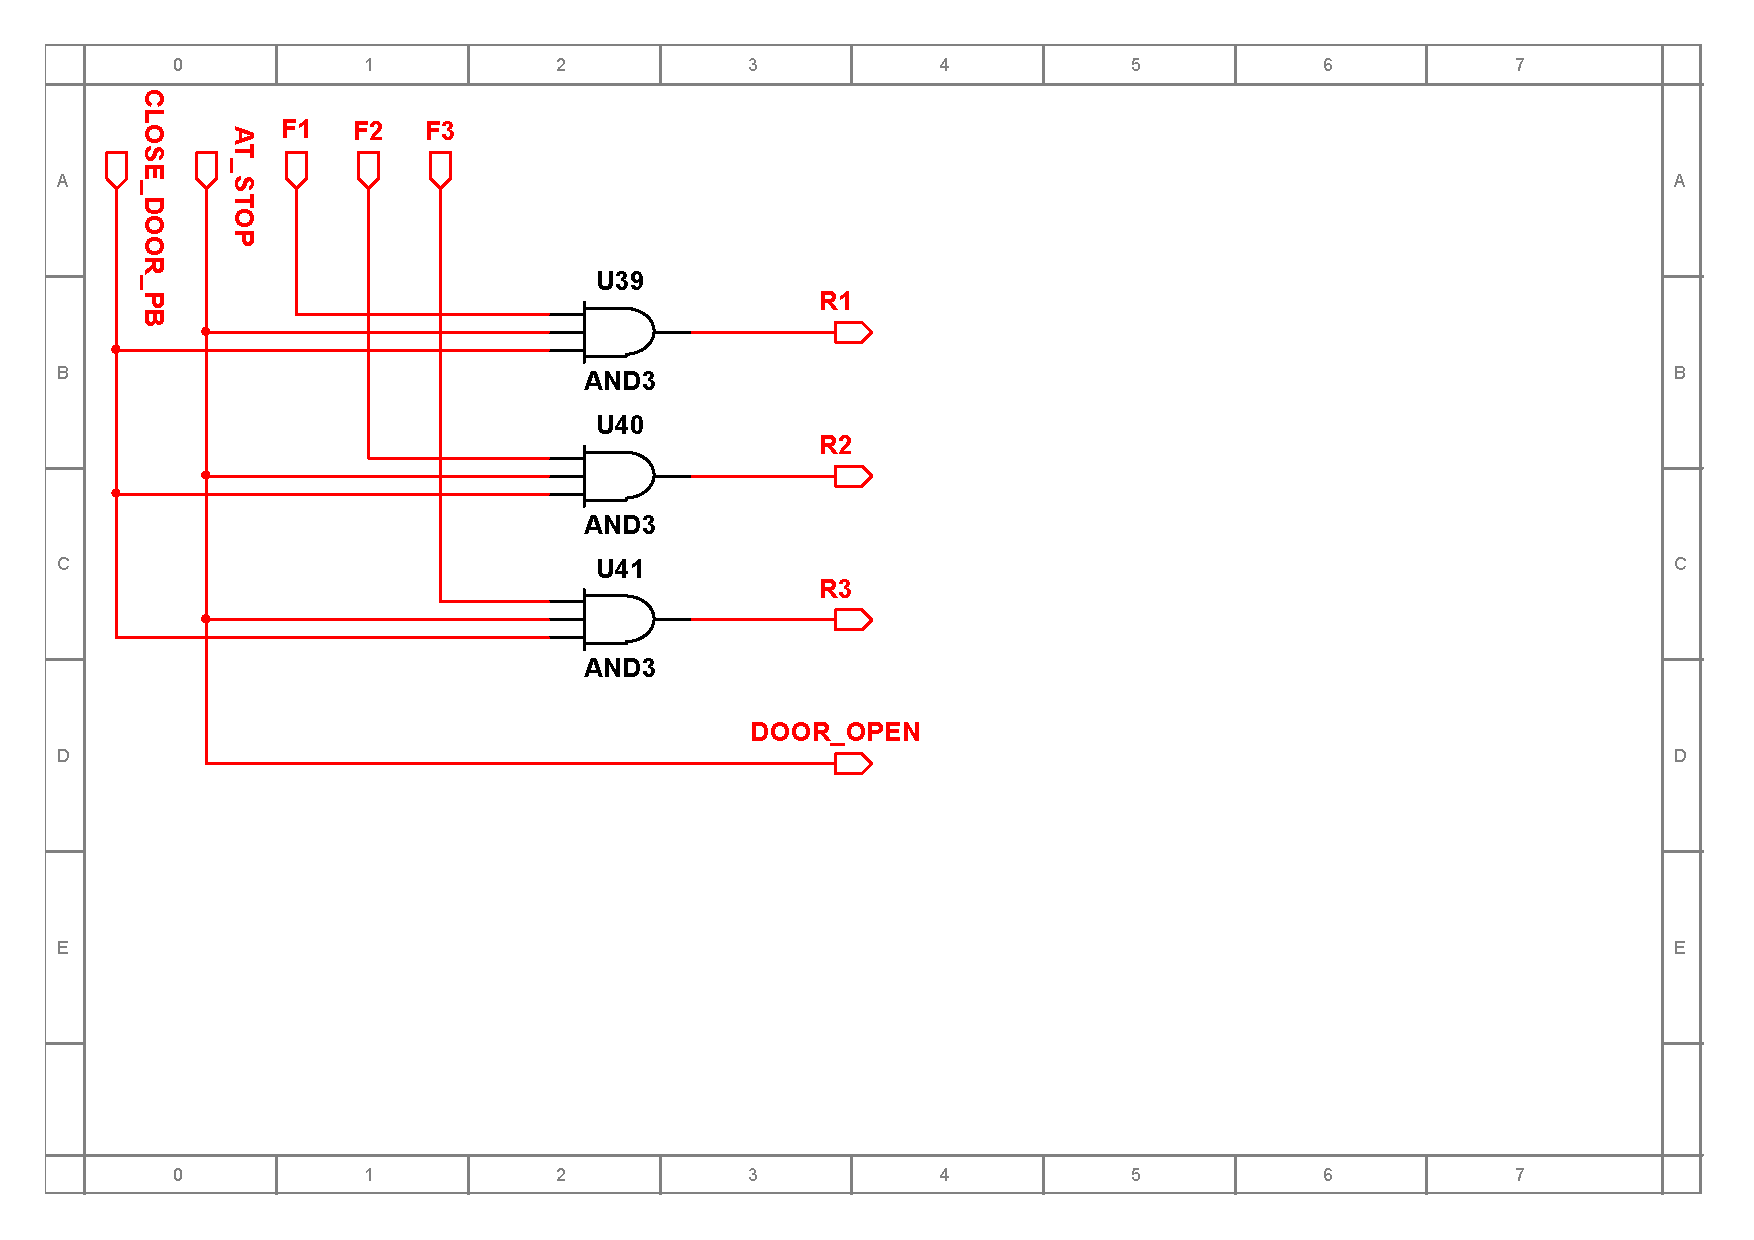
\includegraphics[width=\textwidth]{door_controller_schemat.pdf}
    \caption{Schemat układu kontrolującego obsługę drzwi}
\end{figure}

\pagebreak
\subsection{Kontroler wezwań}
Układ zajmujący się obsługiwaniem wezwań windy w odpowiedniej kolejności.

\subsubsection{Black box}
\begin{figure}[H]
    \centering
    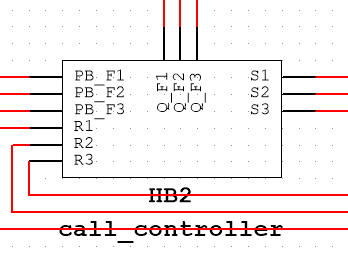
\includegraphics[width=0.6\textwidth]{call_controller.png}
    \caption{Black box układu obsługującego wezwania}
\end{figure}

\subsubsection{Wejścia}
\begin{itemize}
    \item \verb|PB_F1| - sygnał informujący o wciśnięciu przycisku wzywającego windę na 1. piętro.
    \item \verb|PB_F2| - sygnał informujący o wciśnięciu przycisku wzywającego windę na 2. piętro.
    \item \verb|PB_F3| - sygnał informujący o wciśnięciu przycisku wzywającego windę na 3. piętro.
    \item \verb|R1| - sygnał informujący o wykonaniu wezwania na 1. pietro.
    \item \verb|R2| - sygnał informujący o wykonaniu wezwania na 2. pietro.
    \item \verb|R3| - sygnał informujący o wykonaniu wezwania na 3. pietro.
\end{itemize}

\subsubsection{Wyjścia}
\begin{itemize}
    \item \verb|S1| - sygnał obecnie obsługiwanego wezwania na piętro 1.
    \item \verb|S2| - sygnał obecnie obsługiwanego wezwania na piętro 2.
    \item \verb|S3| - sygnał obecnie obsługiwanego wezwania na piętro 3.
    \item \verb|Q_F1| - sygnał informujący, że wezwanie na pietro 1. znajduje się w kolejce do obsłużenia.
    \item \verb|Q_F2| - sygnał informujący, że wezwanie na pietro 2. znajduje się w kolejce do obsłużenia.
    \item \verb|Q_F3| - sygnał informujący, że wezwanie na pietro 3. znajduje się w kolejce do obsłużenia.
\end{itemize}

\subsubsection{Realizacja układu}
\begin{figure}[H]
    \centering
    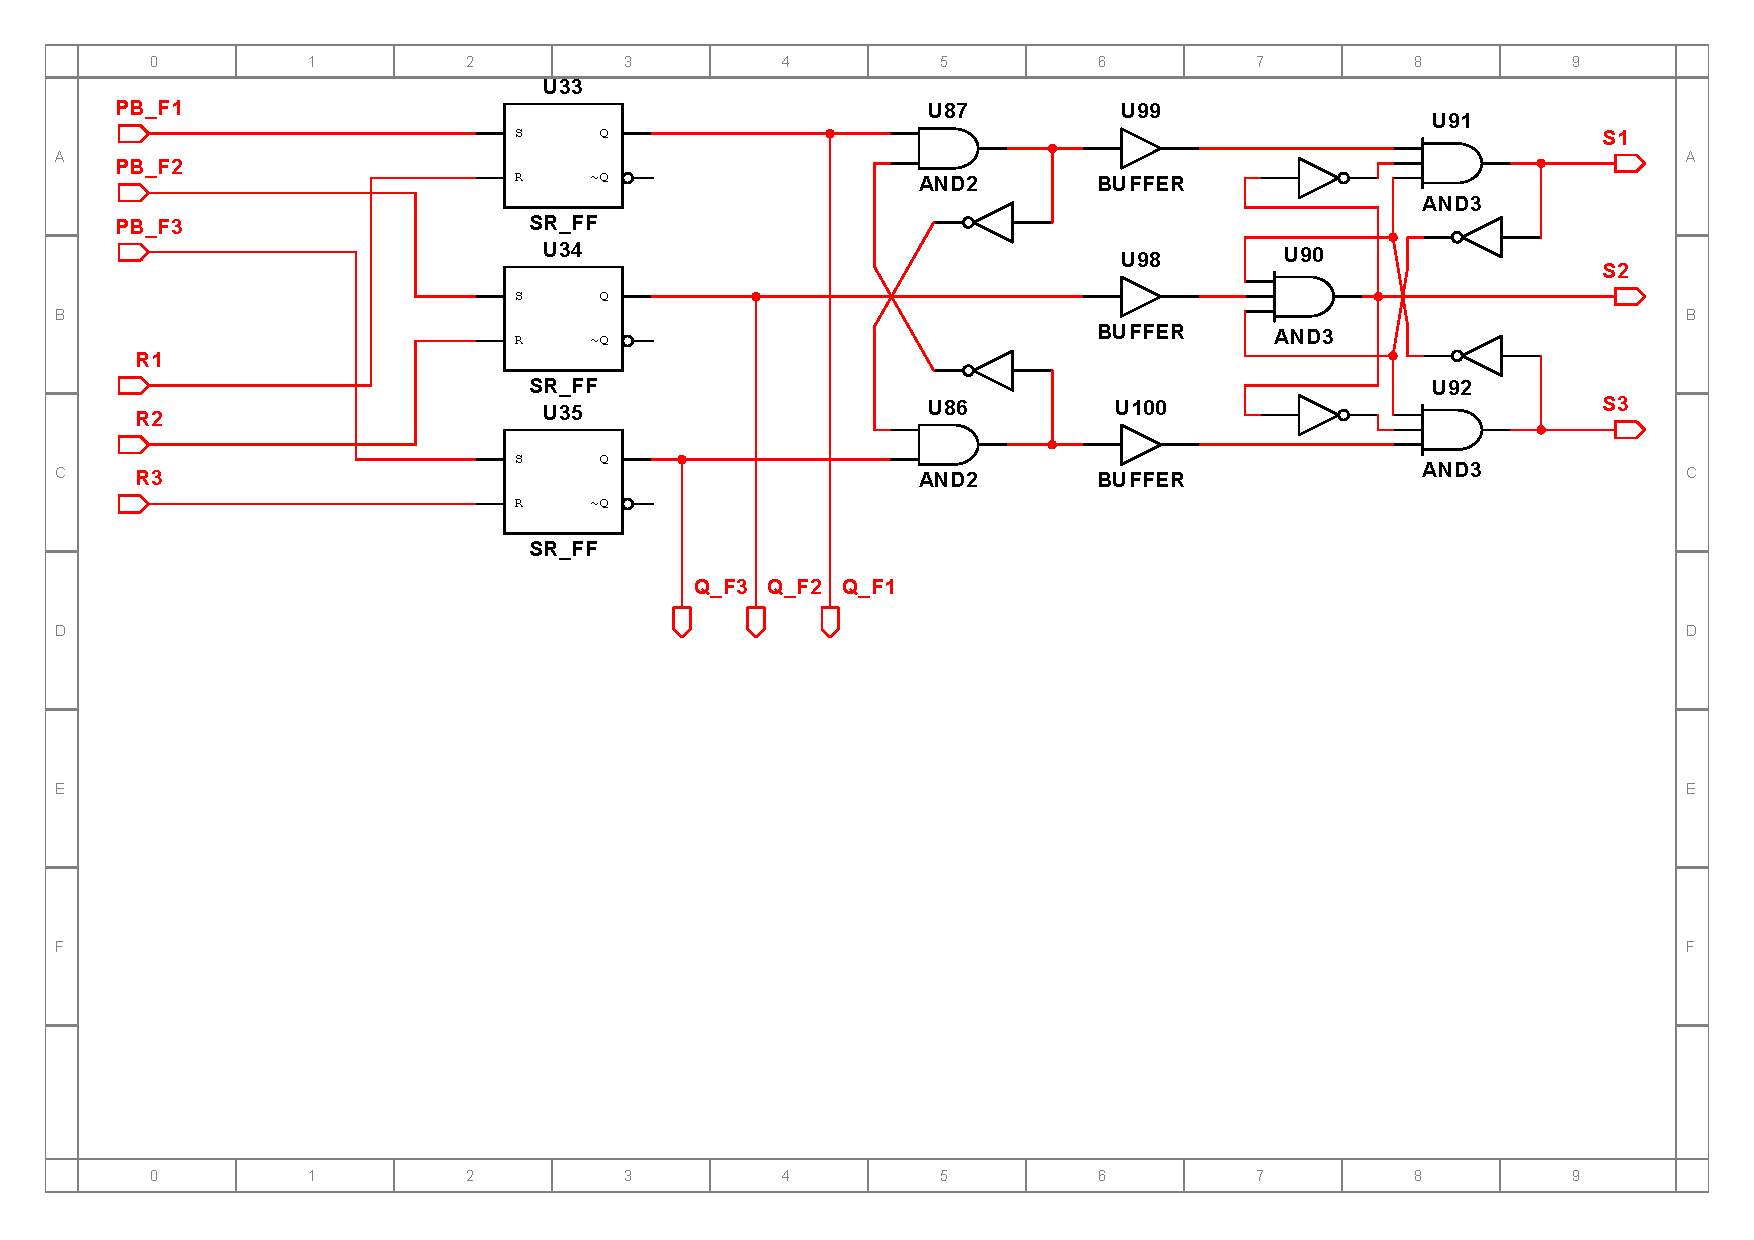
\includegraphics[width=\textwidth]{call_controller.png_schemat.pdf}
    \caption{Schemat układu obsługującego wezwania}
\end{figure}

W naszej implementacji wykorzystaliśmy trzy przerzutniki SR służące do przechowywania
informacji o wezwaniu na dane piętro. Dany przerzutnik jest ustawiany w momencie naciśnięcia odpowiedniego 
przycisku znajdującego się na piętrze lub wewnątrz windy i resetowany po obsłużeniu wezwania.
Kolejną częścią implementacji jest fragment układu, odpowiedzialny za przekazywanie dalej sygnału o wezwaniach.
Sygnały są przekazywane pojedynczo z zachowaniem kolejności w jakiej się pojawiły. 

\subsection{Układ zamykający drzwi}
Układ, który od czasu dotarcia na piętro docelowe odlicza czas po upłynięciu którego wysyła 
sygnał do zamknięcia drzwi. 

\subsubsection{Black box}
\begin{figure}[H]
    \centering
    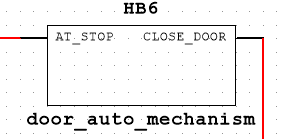
\includegraphics[width=0.6\textwidth]{door_auto_mechanism.png}
    \caption{Black box układu zamykającego drzwi automatycznie}
\end{figure}

\subsubsection{Wejścia}
\begin{itemize}
    \item \verb|AT_STOP| - sygnał wejściowy informujący, że winda znalazła się na piętrze docelowym
\end{itemize}
\subsubsection{Wyjścia}
\begin{itemize}
    \item \verb|CLOSE_DOOR| - sygnał wyjściowy będący sygnałem dla zamknięcia drzwi, jest to krótki puls 
        gdy licznik zakończy działanie.
\end{itemize}
\subsubsection{Realizacja układu}
Do realizacji układu użyliśmy przerzutników D, które generują puls w momencie gdy wartość zmienia stan - wykorzystujemy
je do wygenerowania pulsu startującego licznik oraz do wygenerowania sygnału wyjściowego po zakończeniu działania licznika.
Jako licznik użyliśmy układu typu \verb|555| w trybie monostabilnym (\url{https://en.wikipedia.org/wiki/555_timer_IC#Monostable}).

\begin{figure}[H]
    \centering
    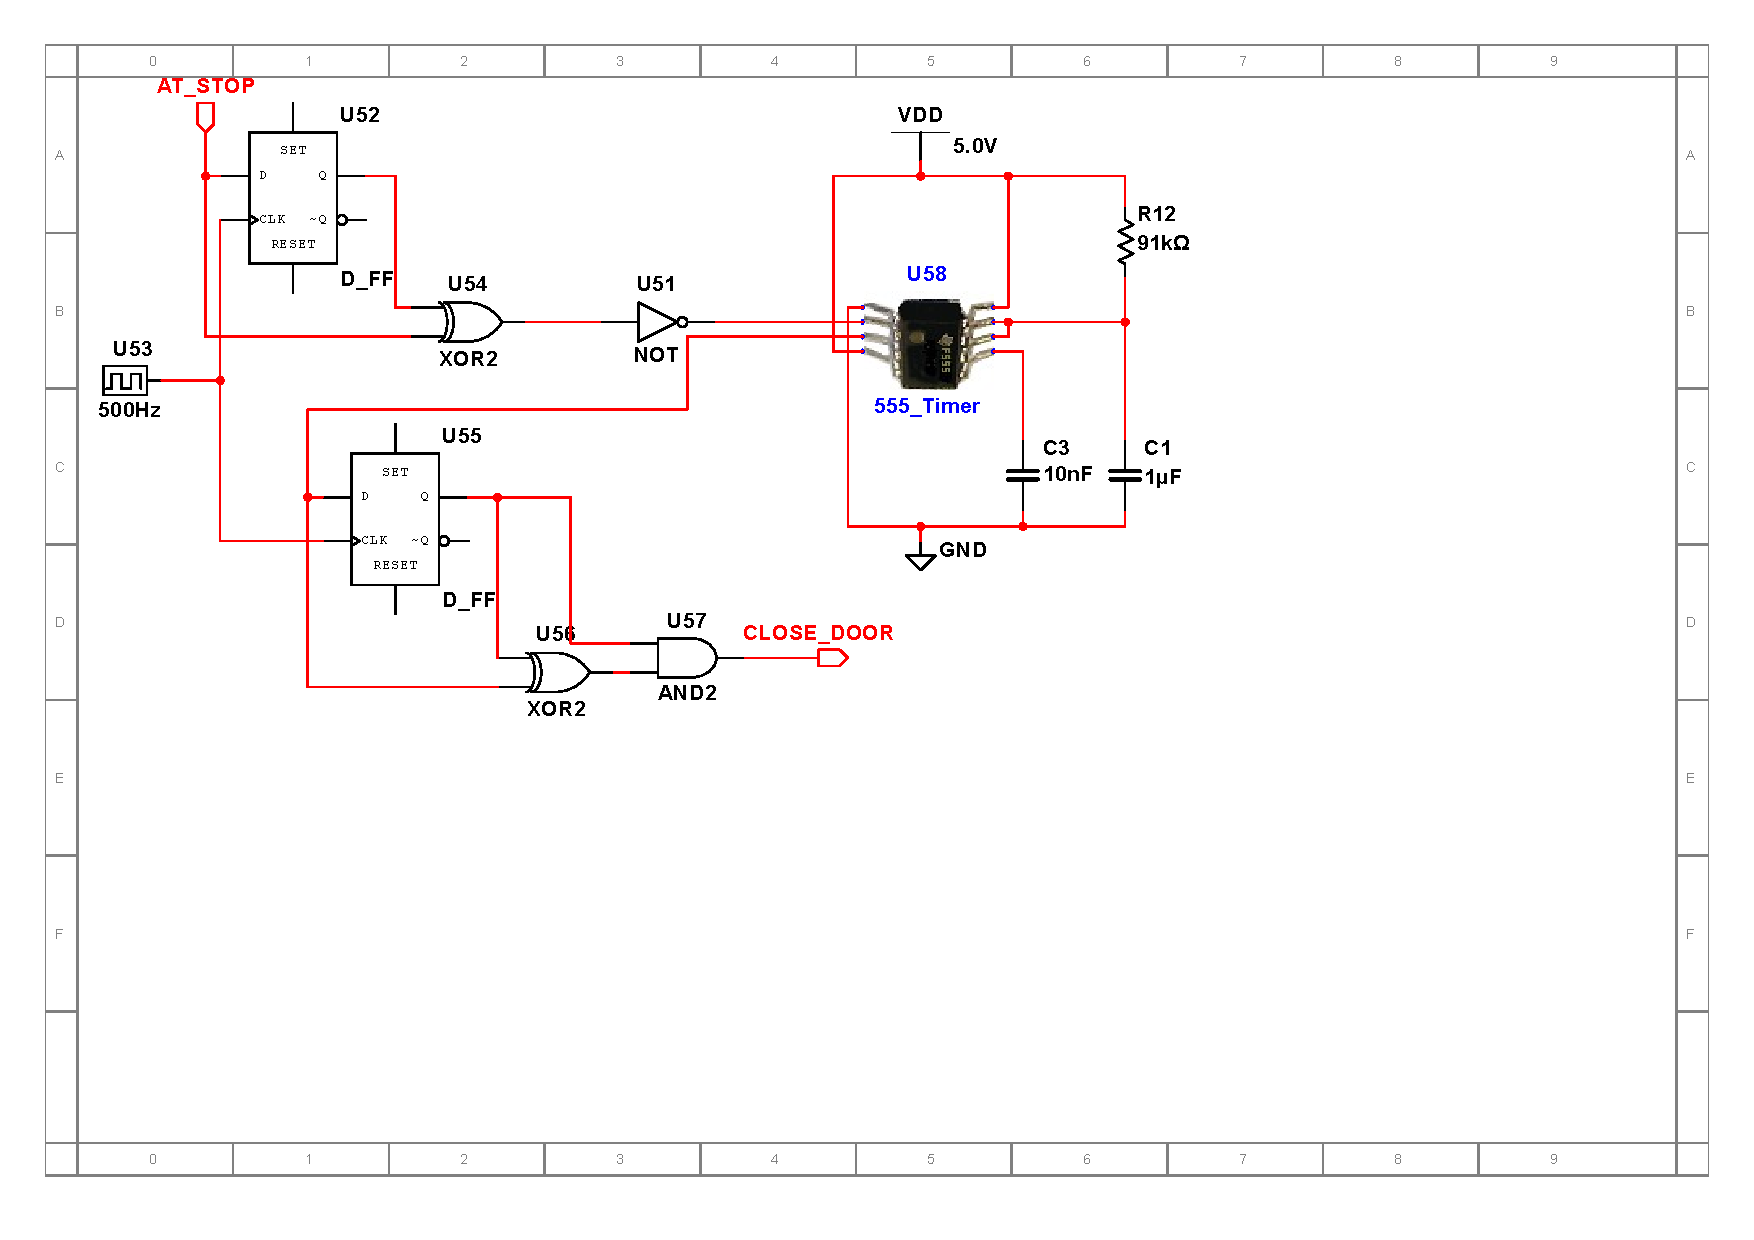
\includegraphics[width=\textwidth]{door_auto_mechanism_schemat.pdf}
    \caption{Schemat układu zamykającego drzwi automatycznie}
\end{figure}

Czas odliczania licznika można regulować za pomocą pojemności kondensatora
\verb|C1| oraz rezystora \verb|R12|. Nasze wartości dobraliśmy z tabelki zamieszczonej na
Wikipedii układu, odpowiadające czasowi odliczania 100ms - co zapewnia dobrze 
widoczny efekt przy tempie symulacji w programie Multisim. Czas można też obliczyć ze wzoru:
\[ t = ln(3) \cdot R_{12} \cdot C_1 \]

\begin{figure}[H]
    \centering
    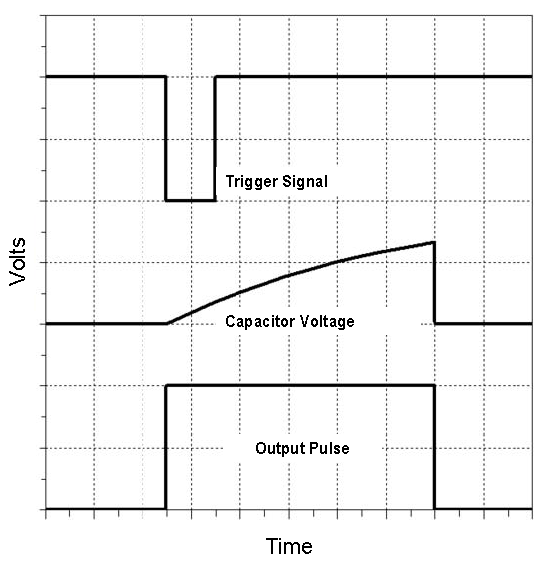
\includegraphics[width=0.3\textwidth]{NE555_Monotable.png}
    \caption{Wykres sygnałów w układzie monostabilnym timera 555}
\end{figure}

Za pomocą przerzutników D generujemy impuls na wejście wyzwalające licznika, a poprzez drugi przerzutnik D generujemy impuls przy opadającym
zboczu wyjścia licznika.

\begin{figure}[H]
    \centering
    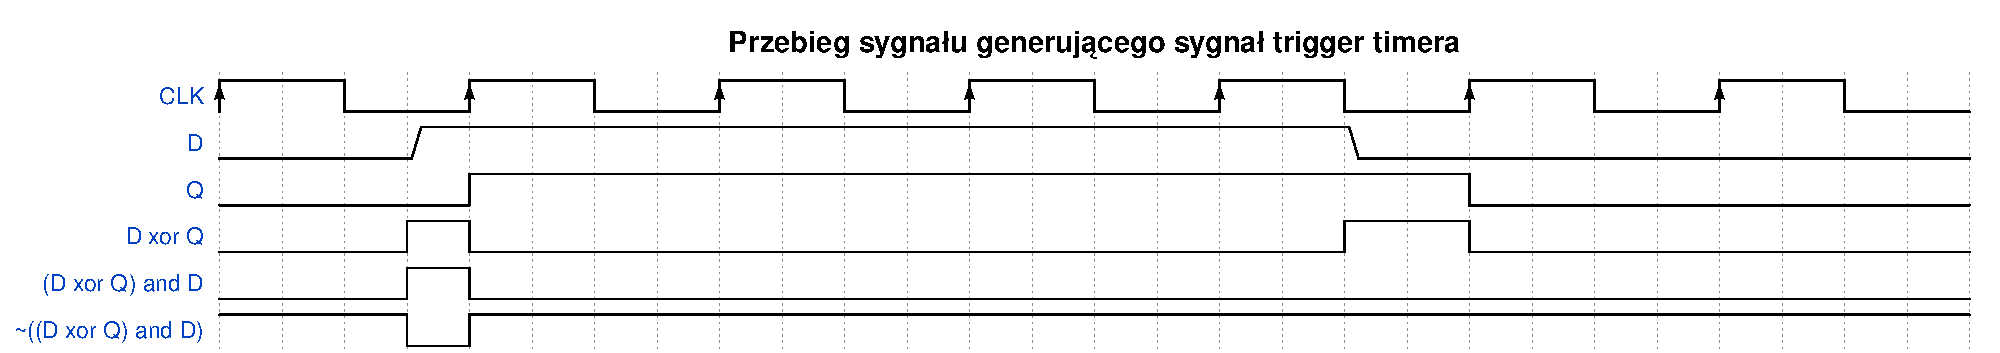
\includegraphics[width=0.8\textwidth]{trigger_waveform.pdf}
    \caption{Przebieg sygnału ilustrujący działanie układu z przerzutnikiem D na wejściu układu}
\end{figure}

\begin{figure}[H]
    \centering
    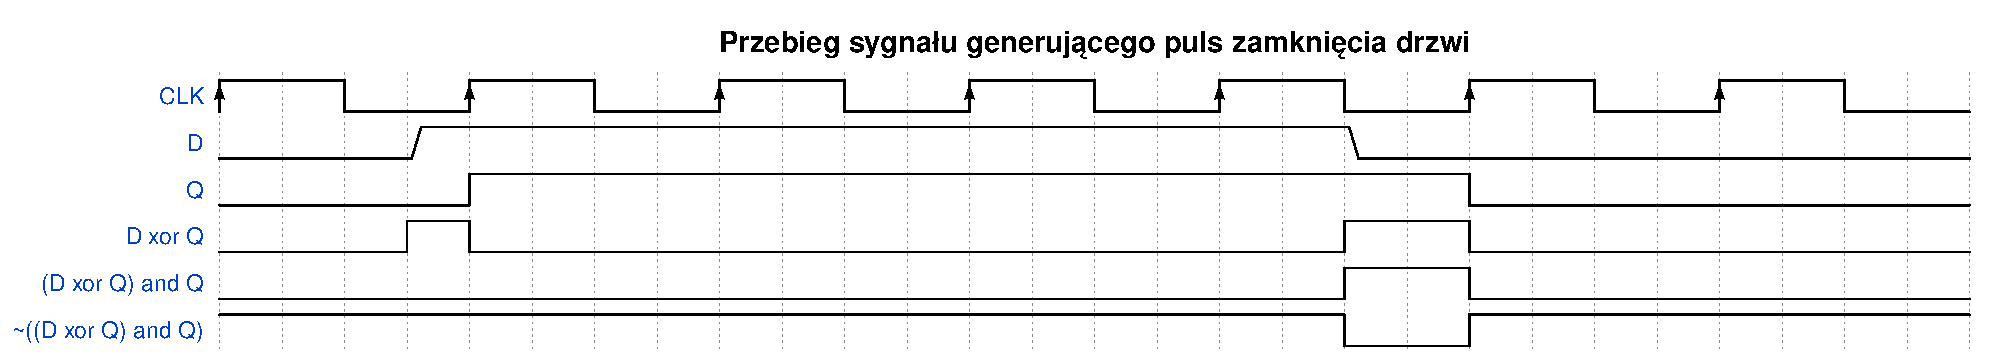
\includegraphics[width=0.8\textwidth]{output_waveform.pdf}
    \caption{Przebieg sygnału ilustrujący działanie układu z przerzutnikiem D na wyjściu układu}
\end{figure}

\pagebreak
\section{Całość układu}
Poniżej przedstawiamy schemat całego systemu z podpiętymi przyciskami i lampkami sygnalizującymi stan windy.
\begin{figure}[H]
    \centering
    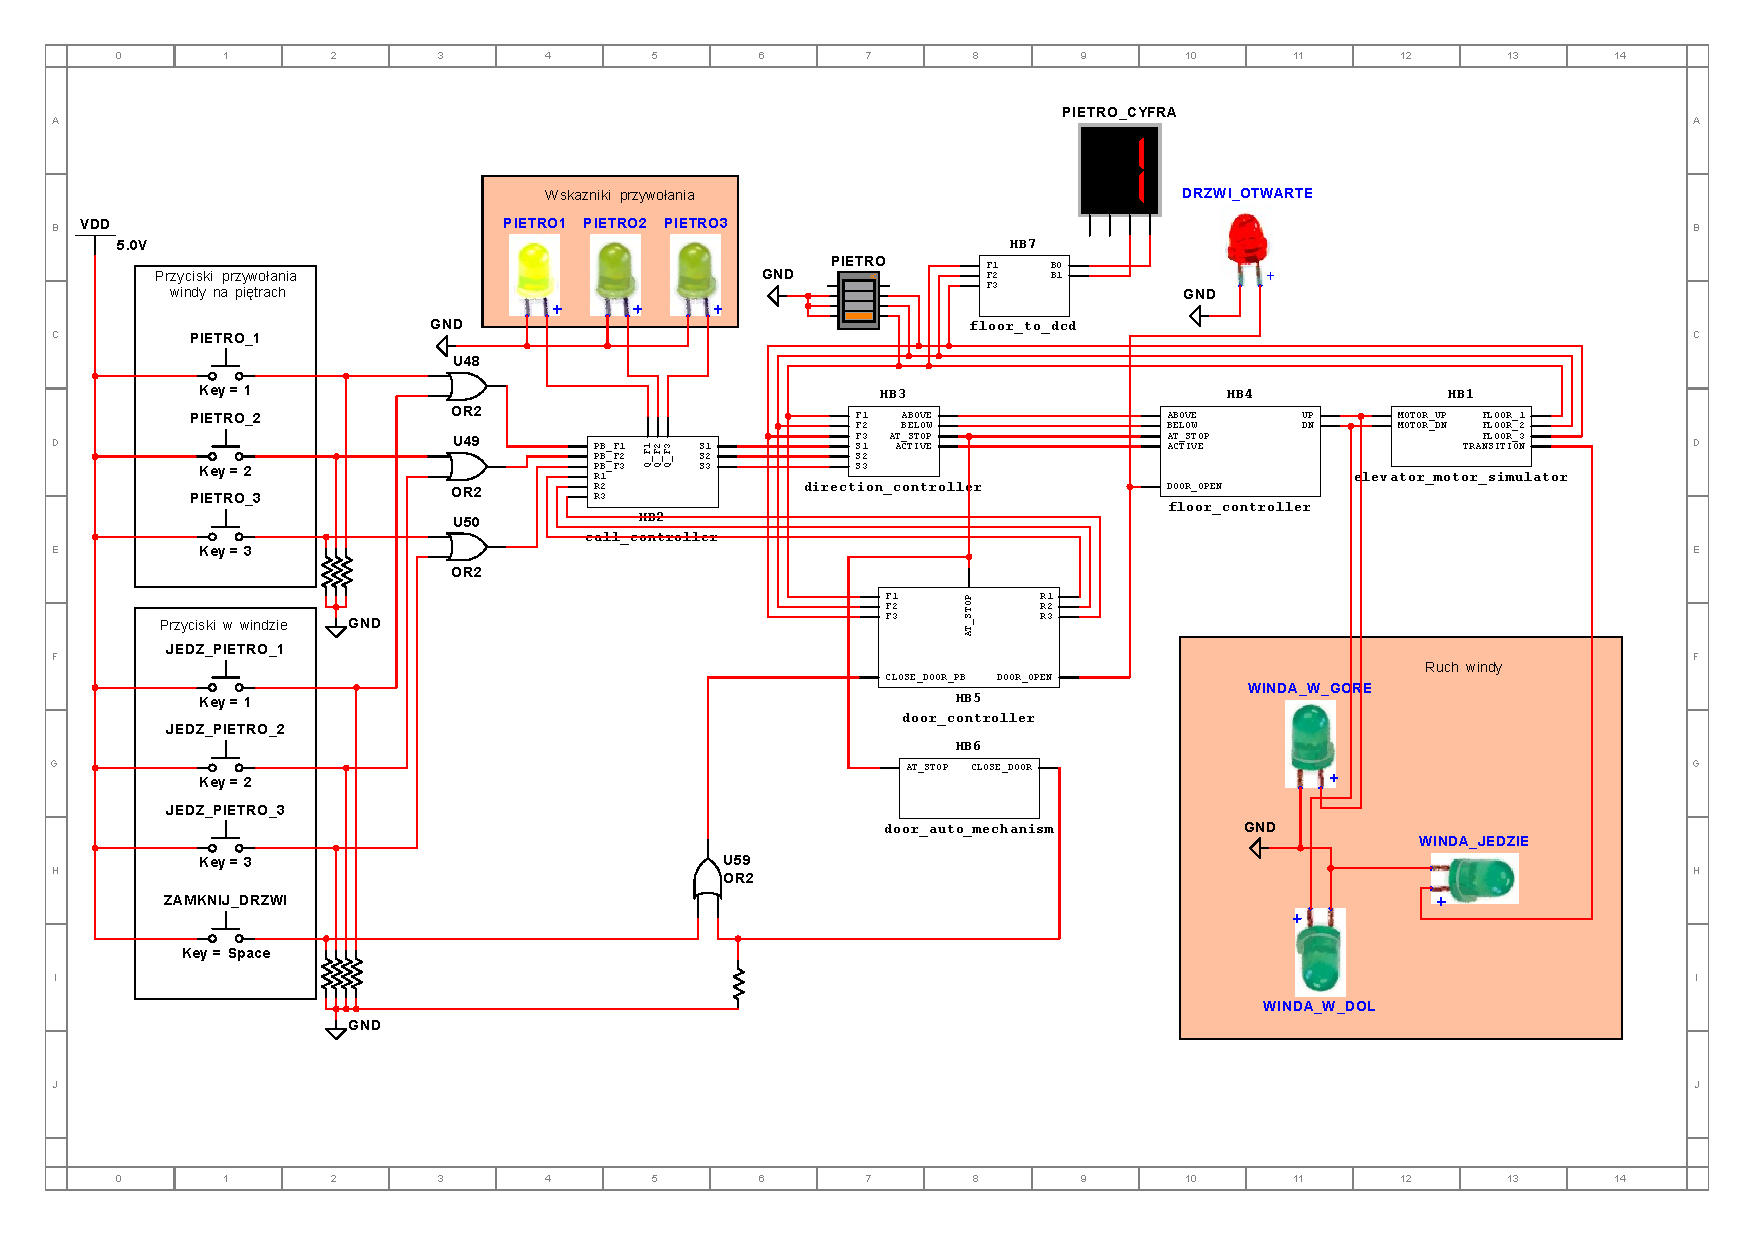
\includegraphics[width=\textwidth]{elevator_system_schemat.pdf}
    \caption{Schemat układu sterującego windą}
\end{figure}
Sterowanie windą odbywa się poprzez 3 przyciski na każdym piętrze przywołujące windę oraz
4 przycisków w kabinie windy: 3 przyciski odpowiadające piętrom docelowym oraz przycisk przyspieszający
zamknięcie drzwi. 

Stan windy sygnalizowany jest przez:
\begin{itemize}
    \item 3 zielone ledy określające stan ruchu windy (czy jedzie, jeśli tak to
w którą stronę)
    \item czerwonego LEDa sygnalizującego otwarcie drzwi
    \item 3 żółtych LED sygnalizujących na które piętro winda jest wezwana
    \item wyświetlacza 7 segmentowego wraz z paskiem LED pokazującym obecne piętro na którym jest winda
\end{itemize}

Winda jest zabezpieczona przed ruszaniem w przypadku otwarcia drzwi. Winda pojedzie tylko wtedy, gdy upłynie
czas automatycznego zamknięcia drzwi lub samemu wciśniemy wcześniej przycisk zamykający drzwi.

\section{Testy}
\subsection{Testy układu floor\_controller}
Aby przetestować układ floor\_controller użyliśmy układu z generatorem słów, który
nadaje dane testowe, komparatorem do wykrywania błędów, analizatorami stanów
logicznych do przedstawienia wejść układu i przebiegu testu oraz przerzutnikiem JK
do sygnalizowania, końcowego wyniku testu.

\begin{figure}[H]
    \centering
    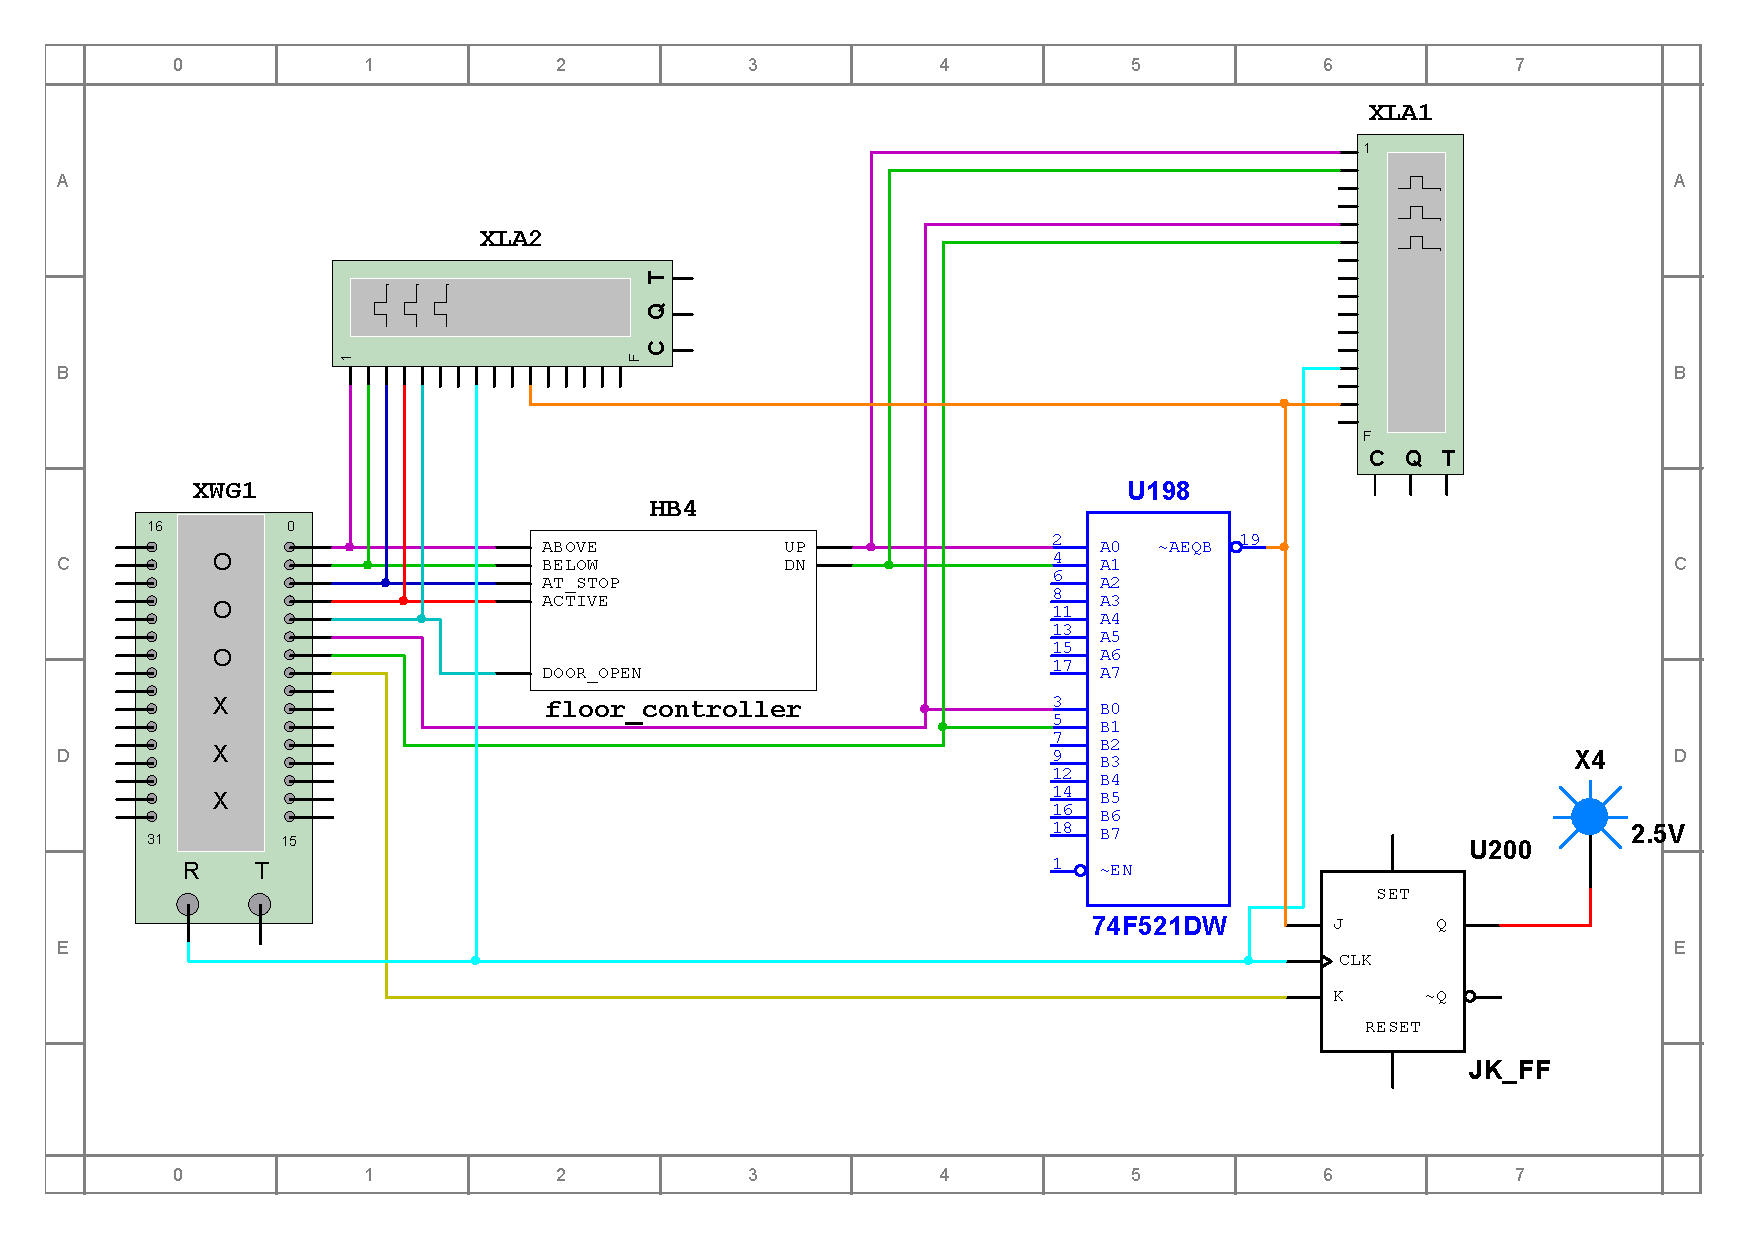
\includegraphics[width=\textwidth]{component_test_floor_controller.pdf}
    \caption{Schemat układu testującego}
\end{figure}

Do łatwego wygenerowania danych testowych wykorzystaliśmy zmodyfikowaną wersję wcześniej przedstawionego
programu do upraszczania formuł logicznych.

\begin{minted}[
    frame=lines,
    framesep=2mm,
    baselinestretch=1.2,
    bgcolor=LightGray,
    fontsize=\footnotesize,
    linenos
]{python}
f = open("floor_controller_test_data.dp", "w")
f.write("Data:\n")
reset_sr = 1
f.write(hex(int(str(bin(1)).removeprefix("0b").rjust(4, '0'), 2)).removeprefix("0x").rjust(8, '0') + "\n")
f.write(hex(int(str(bin(1)).removeprefix("0b").rjust(4, '0'), 2)).removeprefix("0x").rjust(8, '0') + "\n")
f.write(hex(int(str(bin(0)).removeprefix("0b").rjust(4, '0'), 2)).removeprefix("0x").rjust(8, '0') + "\n")
data_count = 3
up = 0
dn = 0
for i in range(32):

    permutation = bin(i).removeprefix("0b").rjust(5, '0')
    
    variables = {
        'DOOR_OPEN': int(permutation[0]),
        'ACTIVE': int(permutation[1]),
        'BELOW': int(permutation[2]),
        'ABOVE': int(permutation[3]),
        'AT_STOP': int(permutation[4])
    }

    set_up = '0'
    reset_up = '0'
    set_dn = '0'
    reset_dn = '0'

    if not variables['ABOVE'] and not variables['BELOW'] and variables['AT_STOP']:
        set_up = '0'
        reset_up = '1'
        set_dn = '0'
        reset_dn = '1'
        up = dn = 0

    elif variables['ACTIVE'] and variables['BELOW'] and not variables['DOOR_OPEN']:
        set_up = '0'
        reset_up = '0'
        set_dn = '1'
        reset_dn = '0'
        dn = 1

    elif variables['ACTIVE'] and variables['ABOVE'] and not variables['DOOR_OPEN']:
        set_up = '1'
        reset_up = '0'
        set_dn = '0'
        reset_dn = '0'
        up = 1

    door_open_b = str(bin(variables['DOOR_OPEN'])).removeprefix("0b")
    active_b = str(bin(variables['ACTIVE'])).removeprefix("0b")
    below_b = str(bin(variables['BELOW'])).removeprefix("0b")
    above_b = str(bin(variables['ABOVE'])).removeprefix("0b")
    at_stop_b = str(bin(variables['AT_STOP'])).removeprefix("0b")
    up_b = str(bin(up)).removeprefix("0b")
    dn_b = str(bin(dn)).removeprefix("0b")

    hex_val = hex(int(dn_b + up_b + door_open_b + active_b + at_stop_b + below_b + above_b, 2))
        .removeprefix("0x").rjust(8, '0')
    f.write(hex_val + "\n")
    data_count += 1

f.write("Initial:\n")
f.write("0000\n")
f.write("Final:\n")
f.write(str(hex(data_count)).capitalize().removeprefix("0x").rjust(4, '0'))

f.close()
\end{minted}

Po zaimportowaniu wygenerowanego pliku do generatora słów, wygląda on następująco:

\begin{figure}[H]
    \centering
    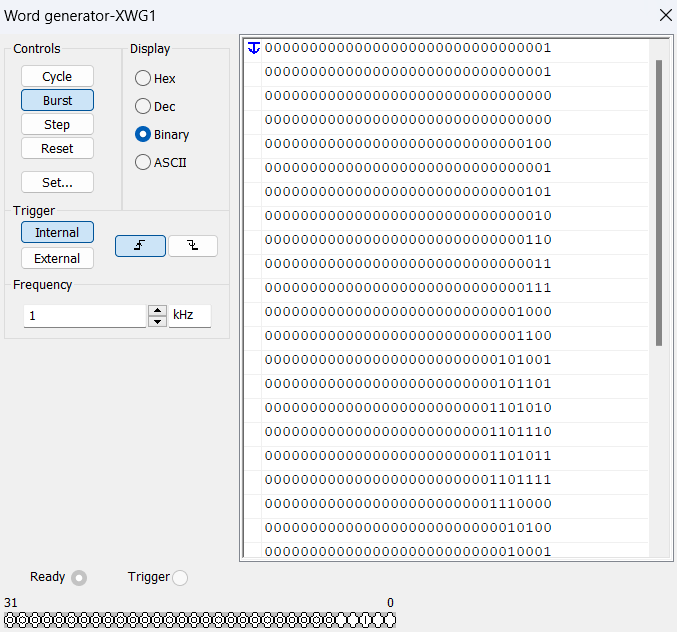
\includegraphics[width=0.6\textwidth]{floor_controller_test_word_generator.png}
    \caption{Dane zaimportowane do generatora słów}
\end{figure}

\pagebreak
Poniżej wynik testu w postaci przebiegu analizatorów stanów logicznych:

\begin{figure}[H]
    \centering
    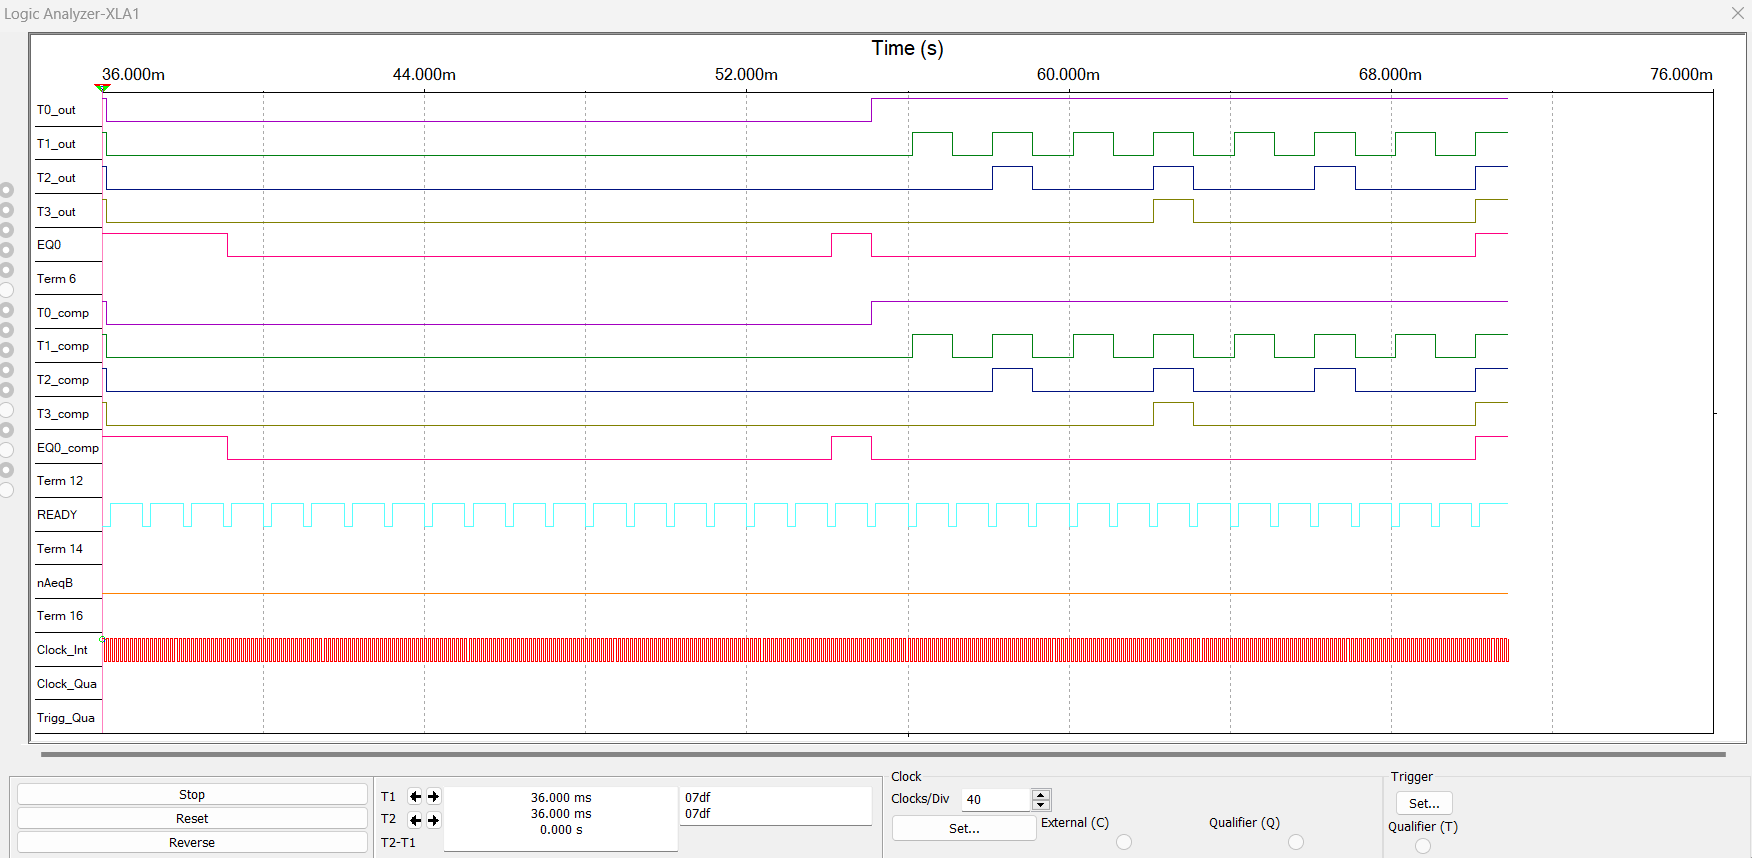
\includegraphics[width=\textwidth]{floor_controller_test_logic_analizer_xla1.png}
    \caption{Przebieg sygnałów w analizatorze stanów logicznych podpiętym do wyjścia układu}
\end{figure}

\begin{figure}[H]
    \centering
    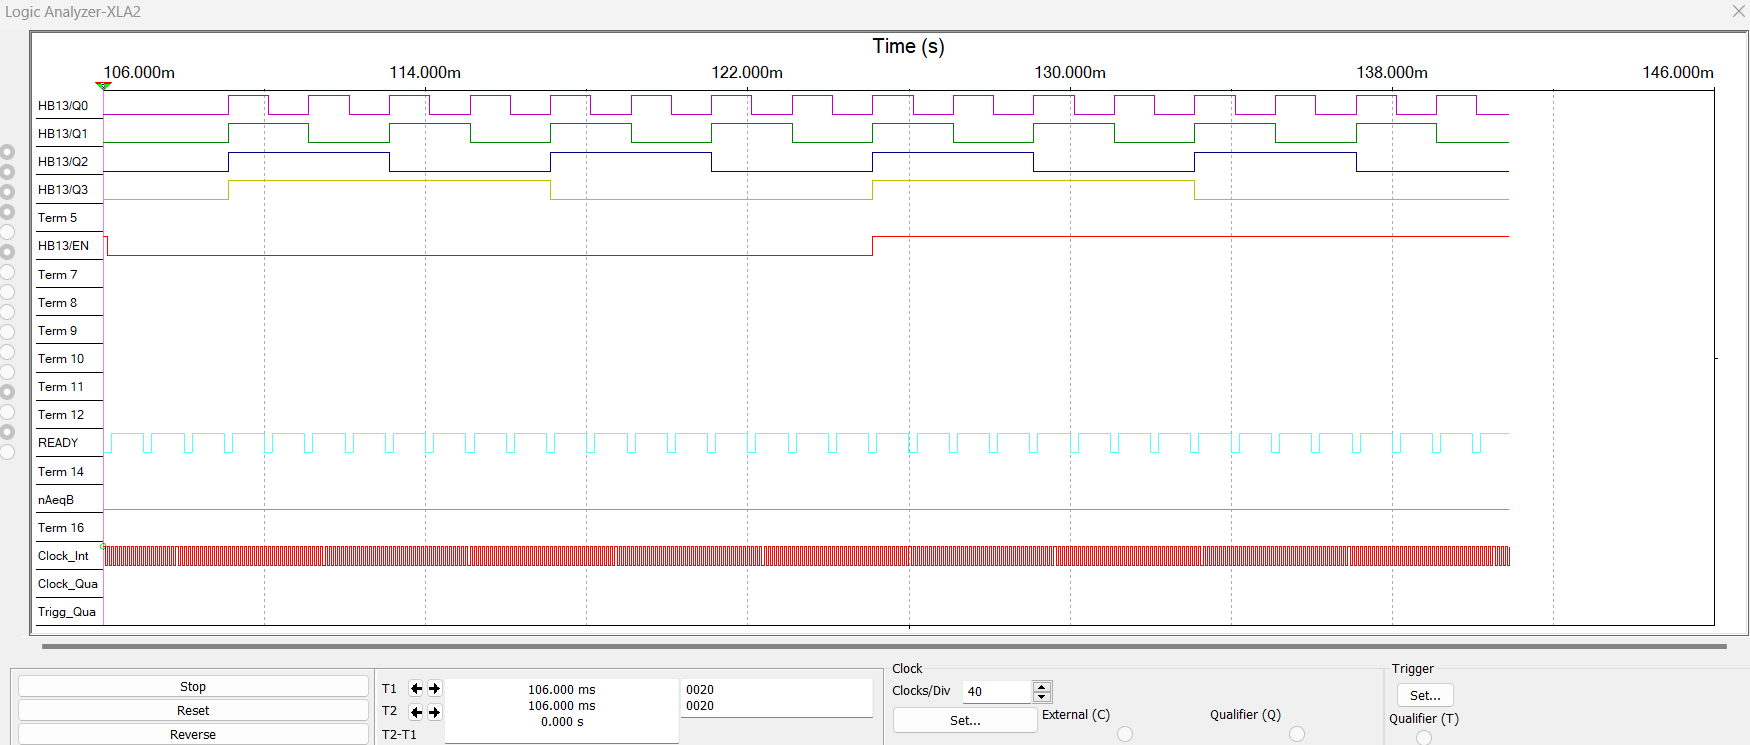
\includegraphics[width=\textwidth]{floor_controller_test_logic_analizer_xla2.png}
    \caption{Przebieg sygnałów w analizatorze stanów logicznych podpiętym do wejścia układu}
\end{figure}

\begin{figure}[H]
    \centering
    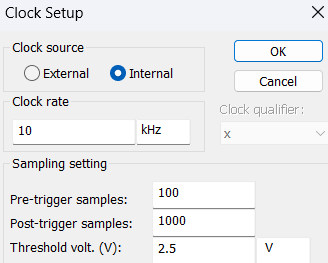
\includegraphics{direction_controller_test_logic_analizer_settings.png}
    \caption{Ustawienia analizatorów}
\end{figure}

\subsection{Testy układu direction\_controller}
Układ testujący dla układu direction\_controller jest analogiczny do poprzedniego.
Tutaj również wykorzystaliśmy generator słów, komparator, dwa analizatory stanów logicznych
i przerzutnik JK. 

\begin{figure}[H]
    \centering
    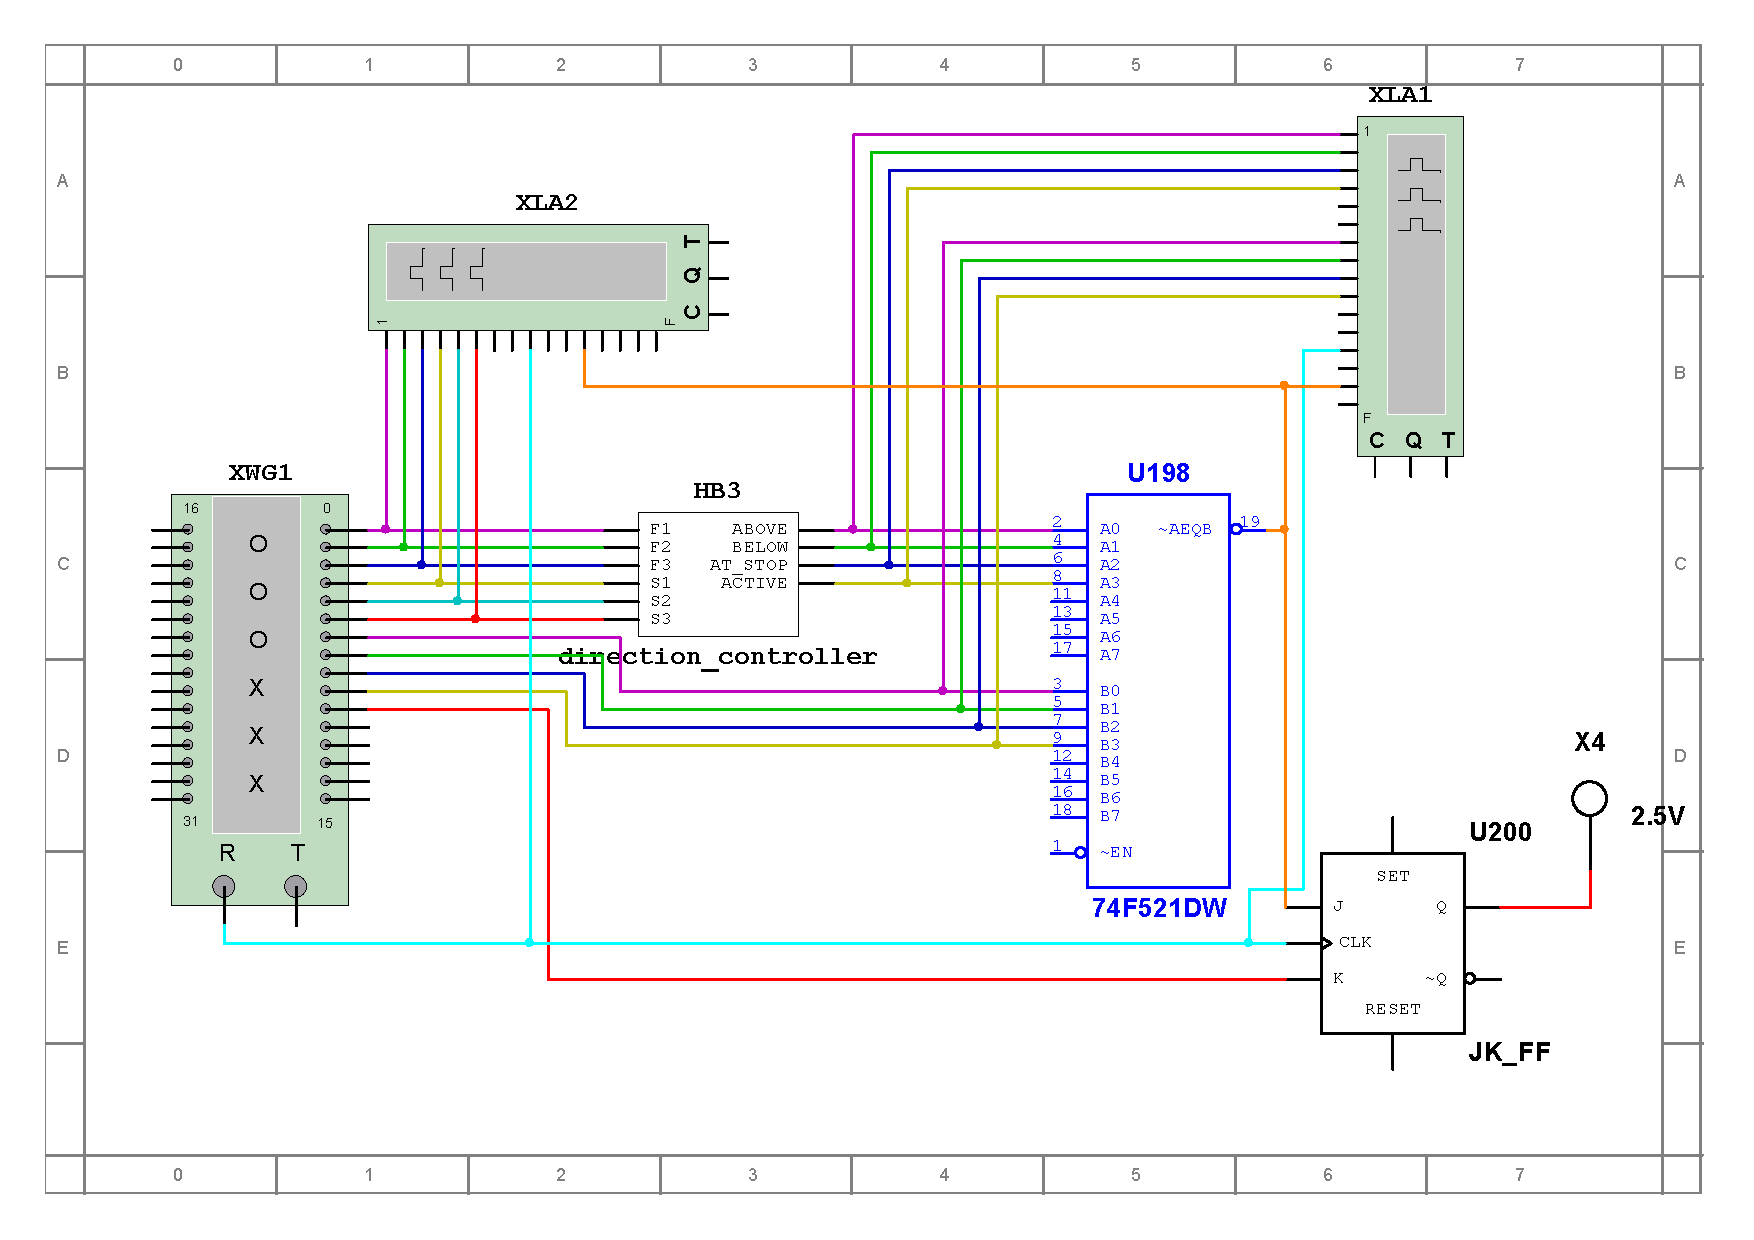
\includegraphics[width=\textwidth]{component_test_direction_controller.pdf}
    \caption{Schemat układu testującego}
\end{figure}

Podobnie jak wcześniej, wykorzystaliśmy zmodyfikowany kod do wyprowadzania formuł.

\begin{minted}[
    frame=lines,
    framesep=2mm,
    baselinestretch=1.2,
    bgcolor=LightGray,
    fontsize=\footnotesize,
    linenos
]{python}
f = open("direction_controller_test_data.dp", "w")
f.write("Data:\n")
reset_sr = 1
f.write(hex(int(str(bin(1)).removeprefix("0b").rjust(4, '0'), 2)).removeprefix("0x").rjust(8, '0') + "\n")
f.write(hex(int(str(bin(1)).removeprefix("0b").rjust(4, '0'), 2)).removeprefix("0x").rjust(8, '0') + "\n")
f.write(hex(int(str(bin(0)).removeprefix("0b").rjust(4, '0'), 2)).removeprefix("0x").rjust(8, '0') + "\n")
data_count = 3
for i in range(64):
    permutation = bin(i).removeprefix("0b").rjust(6, '0')
    
    variables = {
        'F1': int(permutation[0]),
        'F2': int(permutation[1]),
        'F3': int(permutation[2]),
        'S1': int(permutation[3]),
        'S2': int(permutation[4]),
        'S3': int(permutation[5])
    }

    above = '0'
    below = '0'
    at_stop = '0'
    active = '0'

    if variables['F1'] and (variables['S2'] or variables['S3']):
        above = '1'
    
    elif variables['F2'] and variables['S1']:
        below = '1'

    elif variables['F2'] and variables['S3']:
        above = '1'
    
    elif variables['F3']and (variables['S1'] or variables['S2']):
        below = '1'

    if (variables['F1'] and variables['S1']) or (variables['F2'] and variables['S2']) 
            or (variables['F3'] and variables['S3']):
        at_stop = '1'

    if variables['S1'] or variables['S2'] or variables['S3']:
        active = '1'

    F1_b = str(bin(variables['F1'])).removeprefix("0b")
    F2_b = str(bin(variables['F2'])).removeprefix("0b")
    F3_b = str(bin(variables['F3'])).removeprefix("0b")
    S1_b = str(bin(variables['S1'])).removeprefix("0b")
    S2_b = str(bin(variables['S2'])).removeprefix("0b")
    S3_b = str(bin(variables['S3'])).removeprefix("0b")
    above_b = str(bin(int(above))).removeprefix("0b")
    below_b = str(bin(int(below))).removeprefix("0b")
    at_stop_b = str(bin(int(at_stop))).removeprefix("0b")
    active_b = str(bin(int(active))).removeprefix("0b")

    hex_val = hex(int(active_b + at_stop + below_b + above_b + S3_b + S2_b + S1_b + F3_b + F2_b + F1_b, 2))
                    .removeprefix("0x").rjust(8, '0')
    f.write(hex_val + "\n")
    data_count += 1

f.write("Initial:\n")
f.write("0000\n")
f.write("Final:\n")
f.write(str(hex(data_count)).capitalize().removeprefix("0x").rjust(4, '0'))

f.close()
\end{minted}

Po zaimportowaniu wygenerowanego pliku do generatora słów, wygląda on nastę-
pująco:

\begin{figure}[H]
    \centering
    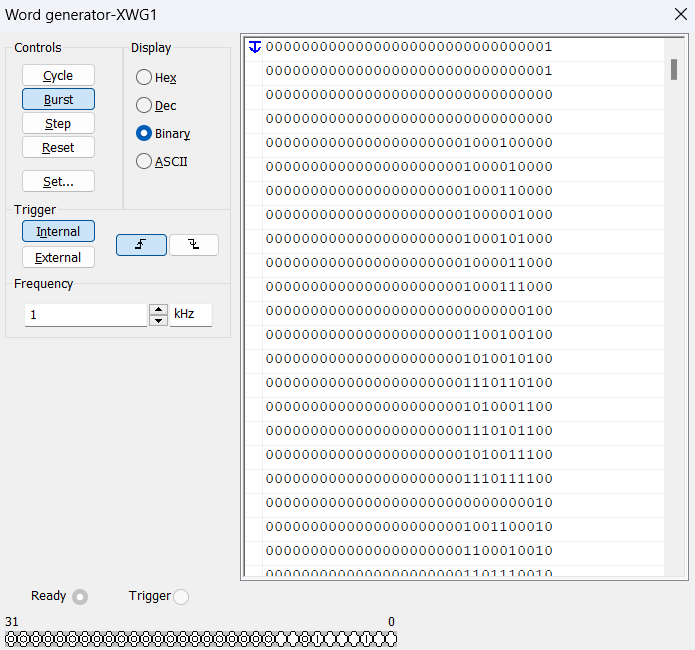
\includegraphics[width=0.6\textwidth]{direction_controller_test_word_generator.png}
    \caption{Dane zaimportowane do generatora słów}
\end{figure}

Poniżej wynik testu w postaci przebiegu analizatorów stanów logicznych:

\begin{figure}[H]
    \centering
    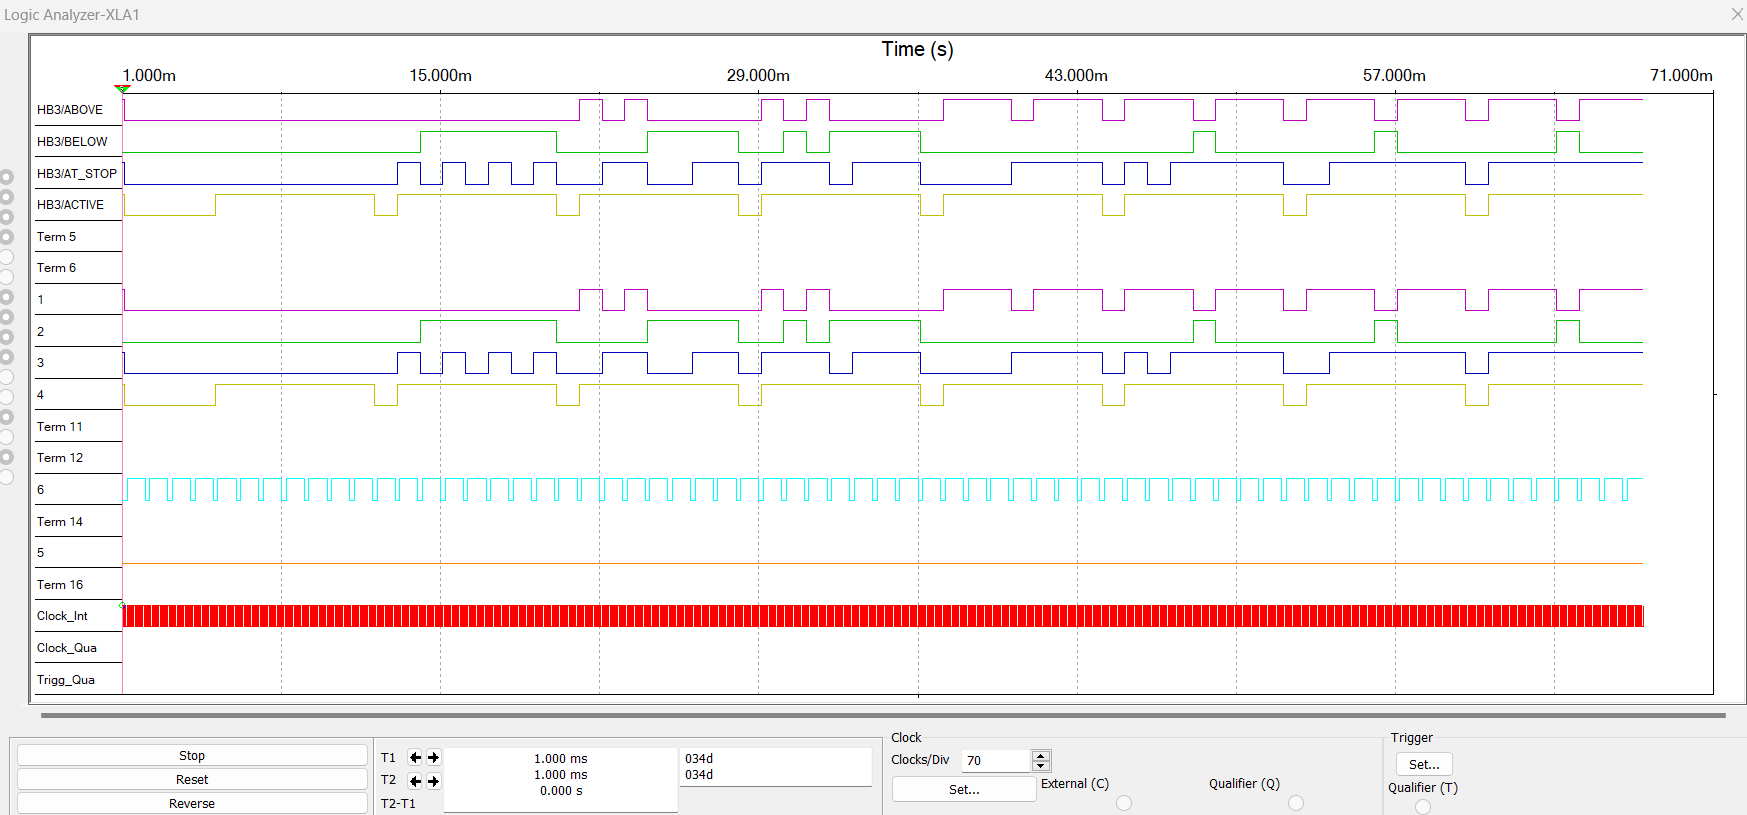
\includegraphics[width=\textwidth]{direction_controller_test_logic_analizer_xla1.png}
    \caption{Przebieg sygnałów w analizatorze stanów logicznych podpiętym do wyjścia układu}
\end{figure}

\begin{figure}[H]
    \centering
    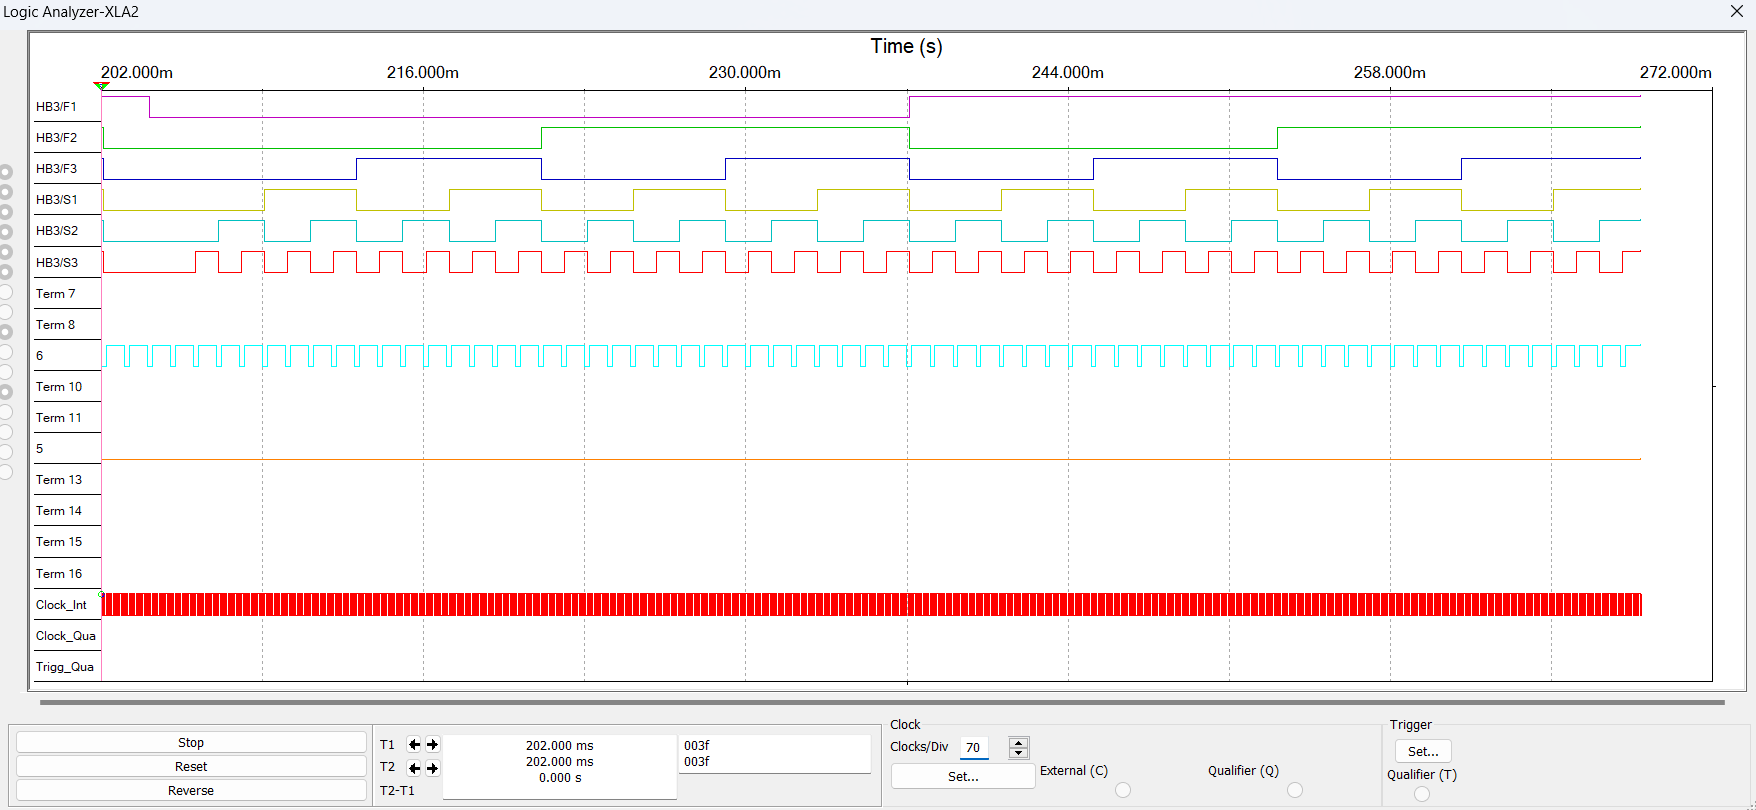
\includegraphics[width=\textwidth]{direction_controller_test_logic_analizer_xla2.png}
    \caption{Przebieg sygnałów w analizatorze stanów logicznych podpiętym do wejścia układu}
\end{figure}

\begin{figure}[H]
    \centering
    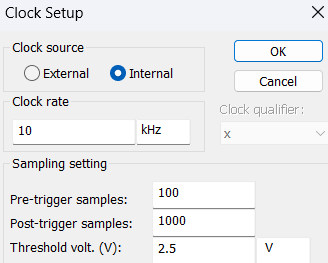
\includegraphics{direction_controller_test_logic_analizer_settings.png}
    \caption{Ustawienia analizatorów}
\end{figure}


\subsection{Testy układu door\_controller}
Układ testujący układu door\_controller jest również całkowicie analogiczny do dwóch poprzednich.

\begin{figure}[H]
    \centering
    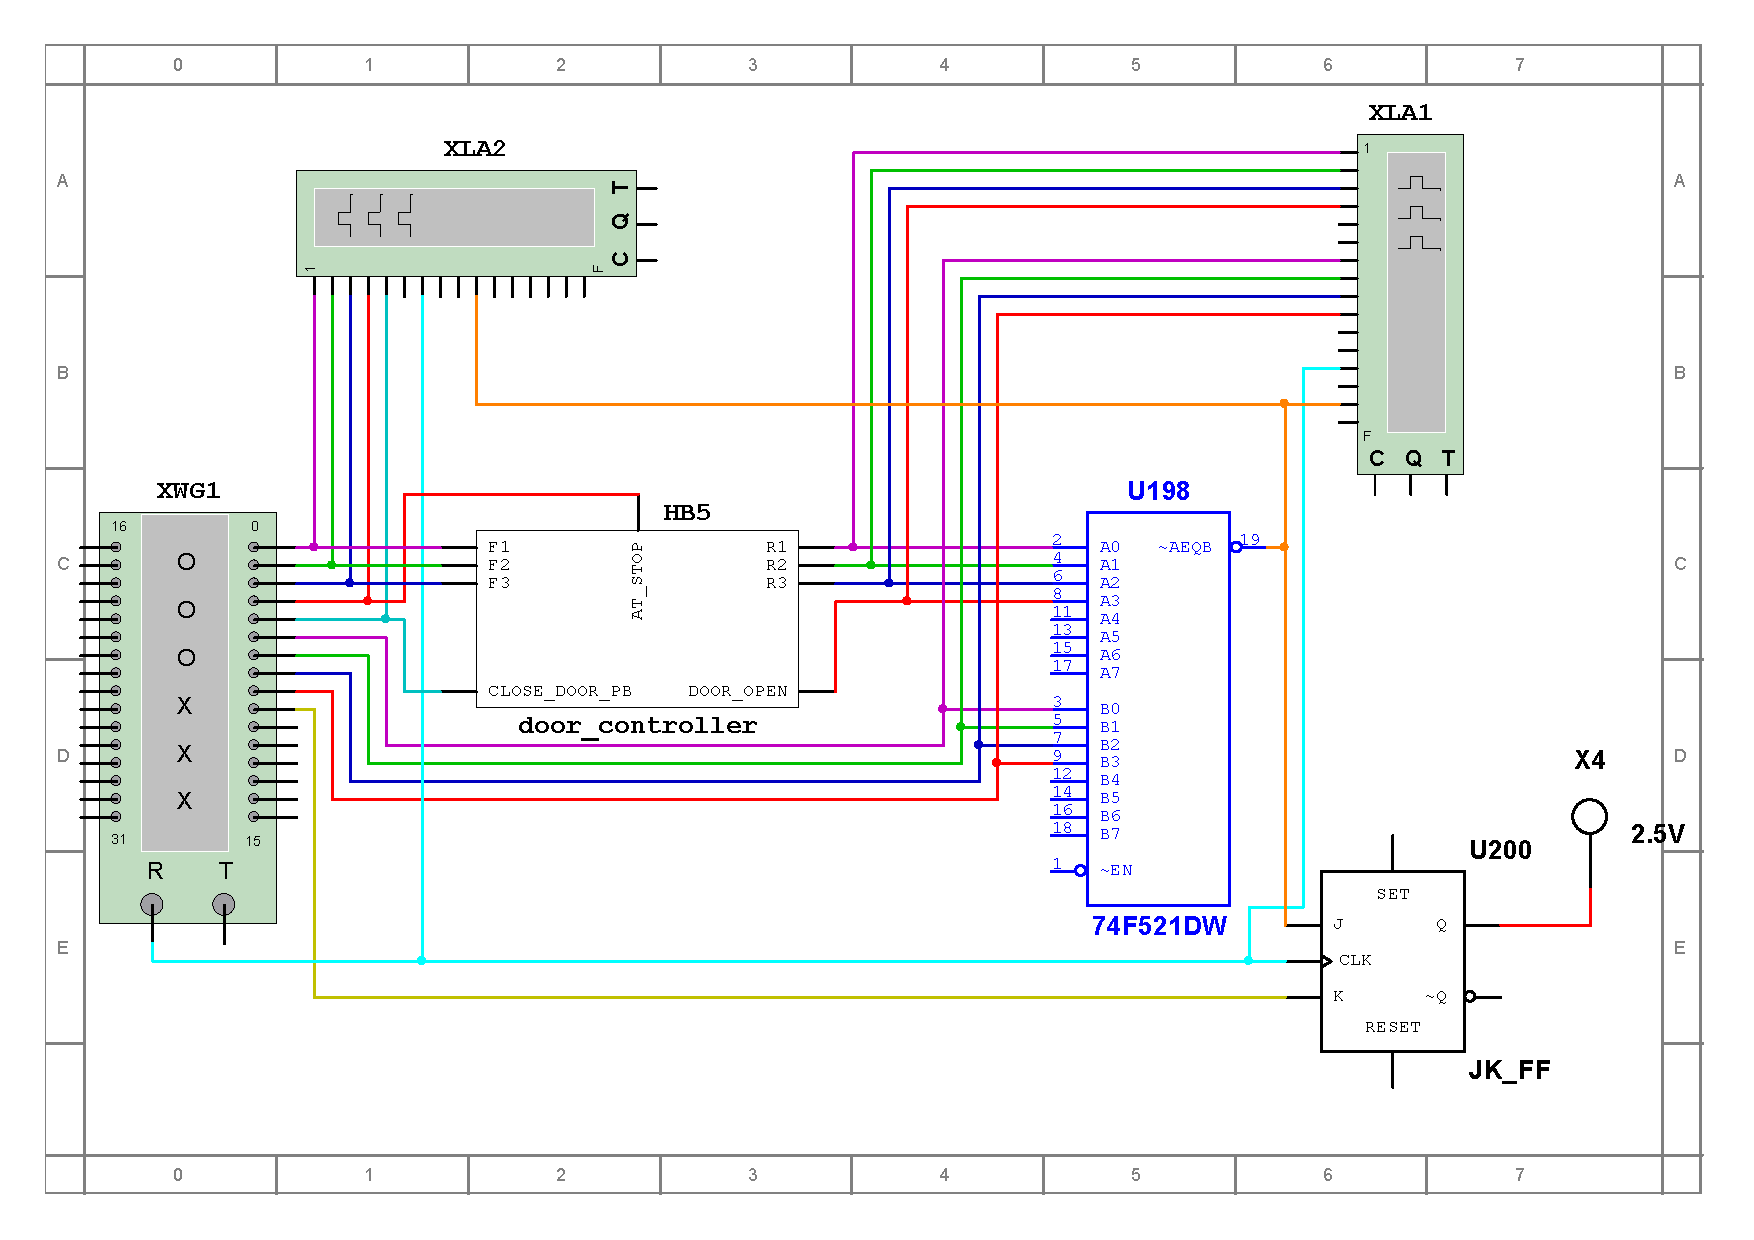
\includegraphics[width=\textwidth]{component_test_door_controller.pdf}
    \caption{Schemat układu testującego}
\end{figure}

Podobnie jak wcześniej, wykorzystaliśmy zmodyfikowany kod do wyprowadzania formuł.

\begin{minted}[
    frame=lines,
    framesep=2mm,
    baselinestretch=1.2,
    bgcolor=LightGray,
    fontsize=\footnotesize,
    linenos
]{python}
f = open("door_controller_test_data.dp", "w")
f.write("Data:\n")
reset_sr = 1
f.write(hex(int(str(bin(1)).removeprefix("0b").rjust(4, '0'), 2)).removeprefix("0x").rjust(8, '0') + "\n")
f.write(hex(int(str(bin(1)).removeprefix("0b").rjust(4, '0'), 2)).removeprefix("0x").rjust(8, '0') + "\n")
f.write(hex(int(str(bin(0)).removeprefix("0b").rjust(4, '0'), 2)).removeprefix("0x").rjust(8, '0') + "\n")
data_count = 3
for i in range(32):
    permutation = bin(i).removeprefix("0b").rjust(5, '0')
    
    variables = {
        'CLOSE_DOOR_PB': int(permutation[0]),
        'AT_STOP': int(permutation[1]),
        'F1': int(permutation[2]),
        'F2': int(permutation[3]),
        'F3': int(permutation[4])
    }

    r1 = '0'
    r2 = '0'
    r3 = '0'
    door_open = '0'

    if variables['AT_STOP']: door_open = '1'
    if variables['AT_STOP'] and variables['CLOSE_DOOR_PB']:
        if variables['F1']: r1 = '1'
        if variables['F2']: r2 = '1'
        if variables['F3']: r3 = '1'

    close_door_pb_b = str(bin(variables['CLOSE_DOOR_PB'])).removeprefix("0b")
    at_stop_b = str(bin(variables['AT_STOP'])).removeprefix("0b")
    F1_b = str(bin(variables['F1'])).removeprefix("0b")
    F2_b = str(bin(variables['F2'])).removeprefix("0b")
    F3_b = str(bin(variables['F3'])).removeprefix("0b")
    r1_b = str(bin(int(r1))).removeprefix("0b")
    r2_b = str(bin(int(r2))).removeprefix("0b")
    r3_b = str(bin(int(r3))).removeprefix("0b")
    door_open_b = str(bin(int(door_open))).removeprefix("0b")

    hex_val = hex(int(door_open_b + r3_b + r2_b + r1_b + close_door_pb_b + at_stop_b + F3_b + F2_b + F1_b, 2))
                    .removeprefix("0x").rjust(8, '0')
    f.write(hex_val + "\n")
    data_count += 1

f.write("Initial:\n")
f.write("0000\n")
f.write("Final:\n")
f.write(str(hex(data_count)).capitalize().removeprefix("0x").rjust(4, '0'))

f.close()
\end{minted}

Po zaimportowaniu wygenerowanego pliku do generatora słów, wygląda on następująco:

\begin{figure}[H]
    \centering
    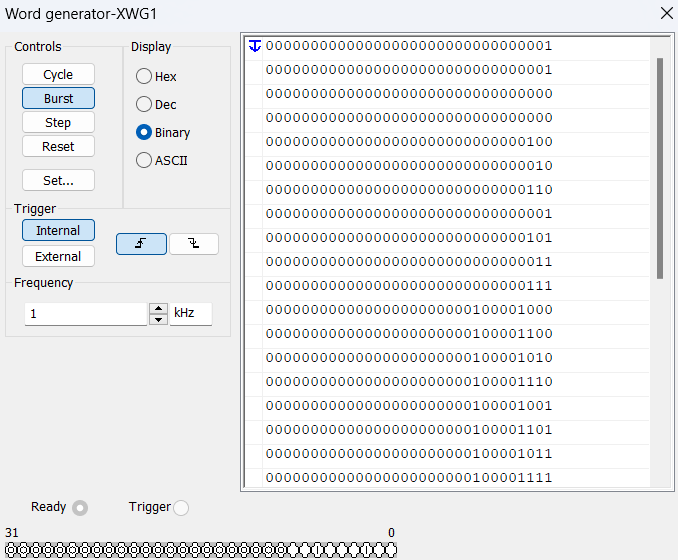
\includegraphics[width=0.6\textwidth]{door_controller_test_word_generator.png}
    \caption{Dane zaimportowane do generatora słów}
\end{figure}

Poniżej wynik testu w postaci przebiegu analizatorów stanów logicznych:

\begin{figure}[H]
    \centering
    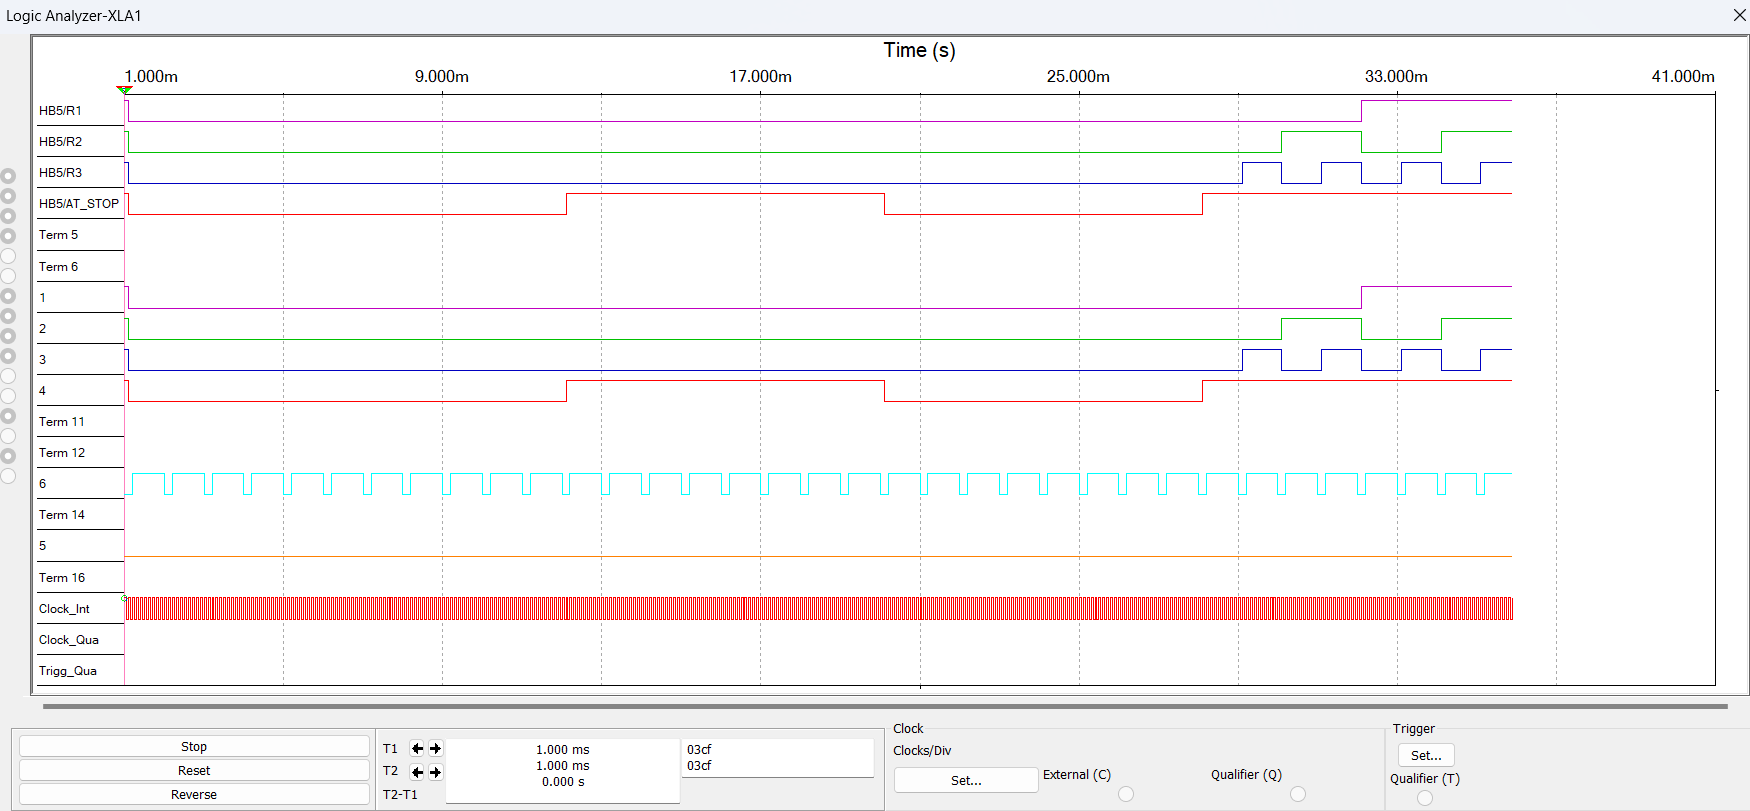
\includegraphics[width=\textwidth]{door_controller_test_logic_analizer_xla1.png}
    \caption{Przebieg sygnałów w analizatorze stanów logicznych podpiętym do wyjścia układu}
\end{figure}

\begin{figure}[H]
    \centering
    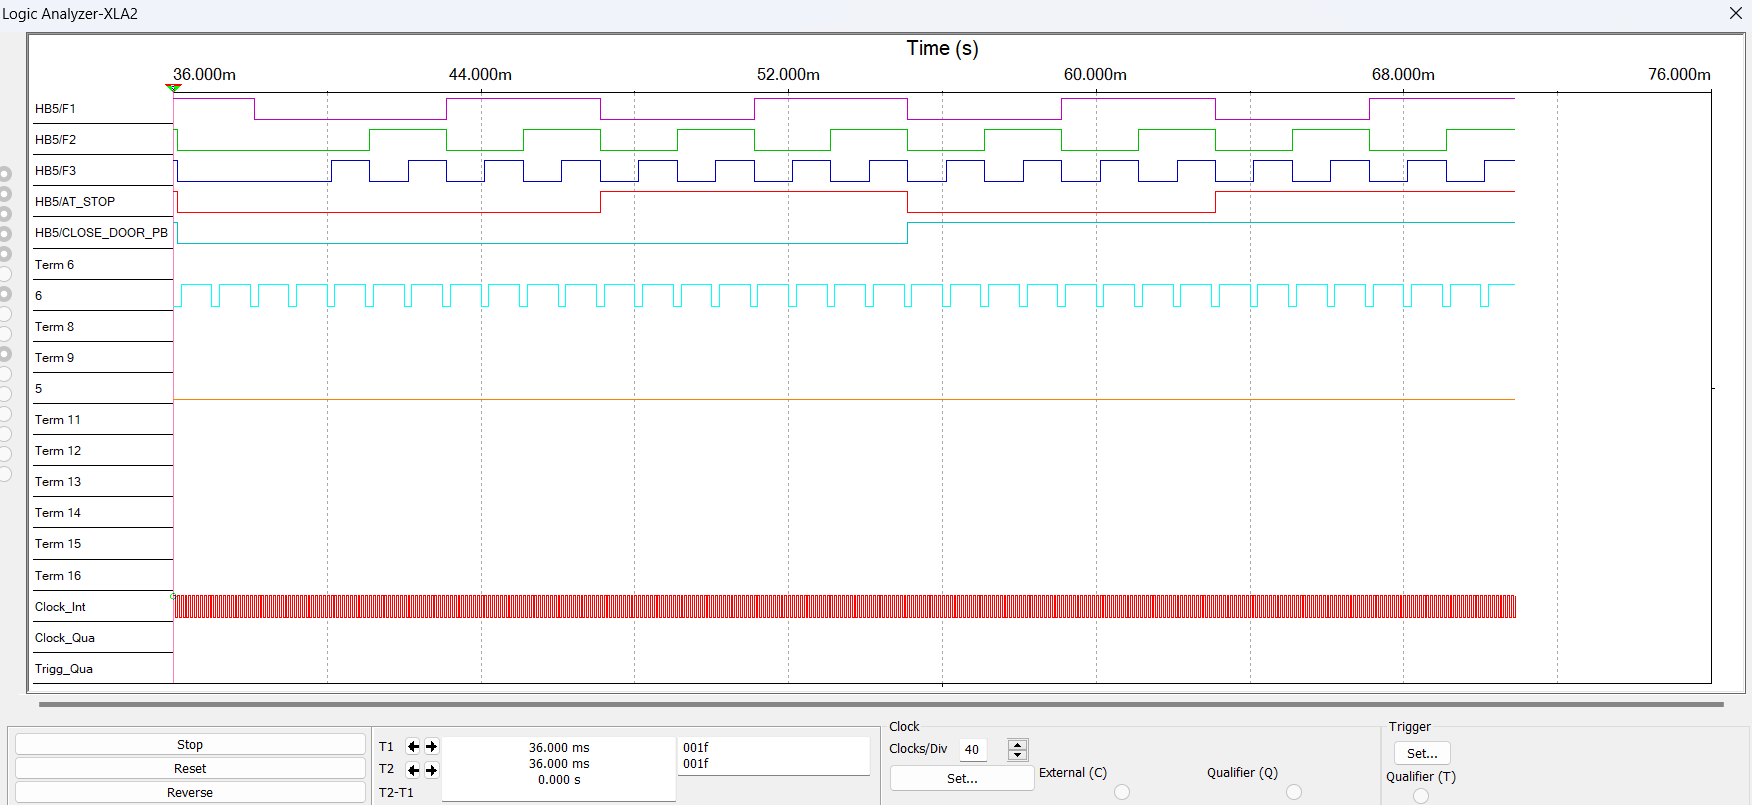
\includegraphics[width=\textwidth]{door_controller_test_logic_analizer_xla2.png}
    \caption{Przebieg sygnałów w analizatorze stanów logicznych podpiętym do wejścia układu}
\end{figure}

\begin{figure}[H]
    \centering
    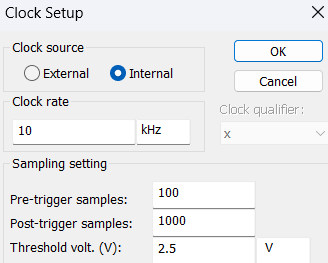
\includegraphics{direction_controller_test_logic_analizer_settings.png}
    \caption{Ustawienia analizatorów}
\end{figure}

\section{Zastosowania}
\begin{itemize}
    \item Oczywistym rozwiązaniem jest zastosowanie windy w trzykondygnacyjnym budynku. Jest to szczególnie potrzebne w miejscach do których uczęszczają osoby niepełnosprawne lub starsze.
 W miejsce segmentu odpowiedzialnego za symulację windy,
  wprowadzono rzeczywistą windę wyposażoną w wbudowane czujniki określające czy na danym piętrze znajduje się winda.
     Informacje te są następnie przekazywane do układu sterującego silnikiem windy.
      Układ ten, opierając się na danych z czujników oraz sygnałach z przycisków na poszczególnych piętrach,
       generuje odpowiednie komendy dotyczące kierunku poruszania się windy.
       
       \begin{figure}[H]
        \centering
        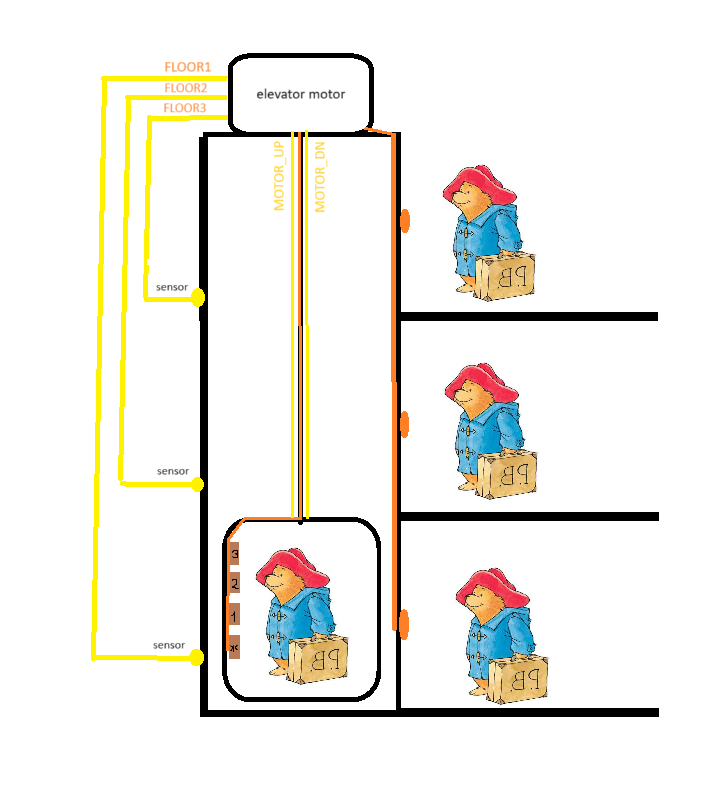
\includegraphics[width=\textwidth]{elevator.png}
        \caption{schemat windy}
    \end{figure}
    \item nie oznacza to jednak, że takiego układu nie można zastosować poza mechanizmem windy. Można zastosować to również w wózku na szynach,
 który służyłby do pomocy w przenoszeniu ciężkich rzeczy. Tak samo jak w powyższym przykładzie segment odpowiedzialny za symulacje windy został zastąpiony wózkiem.
\end{itemize}

\begin{figure}[H]
    \centering
    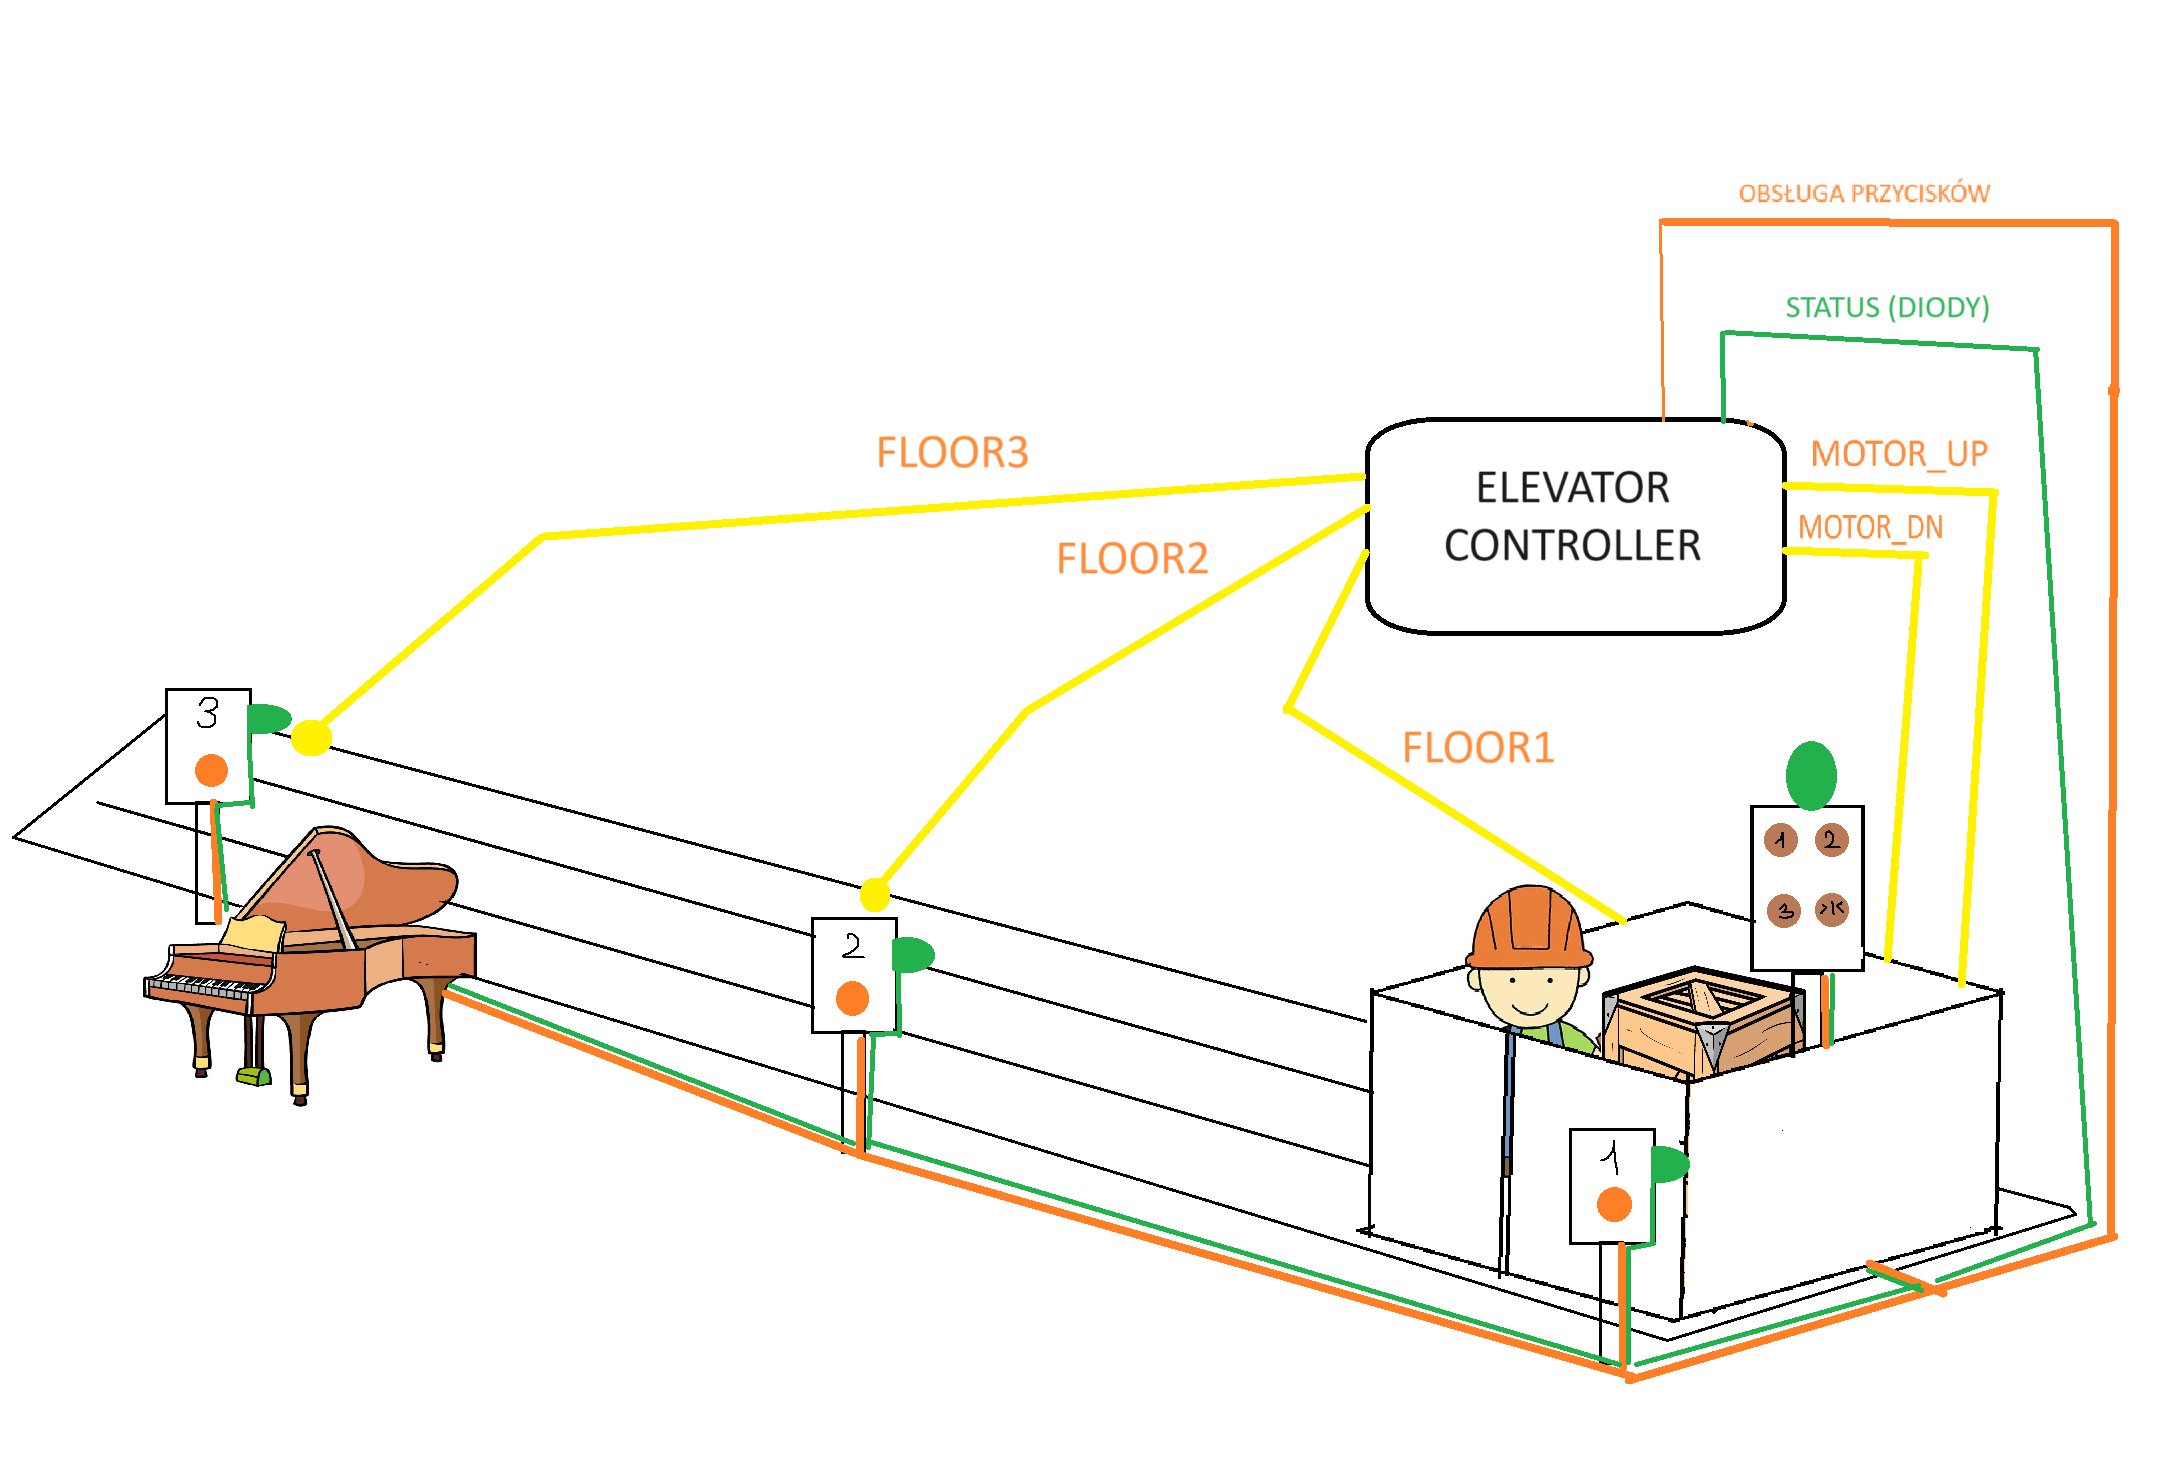
\includegraphics[width=\textwidth]{nieelevator.png}
    \caption{schemat wózka na szynach}
\end{figure}


\section{Wnioski}
Inne sposoby realizacji które rozważaliśmy:

\begin{itemize} 
\item Próbowaliśmy stworzyć automat skończony, opisujący stany w których aktualnie znajduje się winda. 
Niestety implementacja tego w Multisimie była nieefektywna i 
skomplikowana, co sprawiło, że zrezygnowaliśmy z tego pomysłu.
Automat ten byłby łatwiejszy przy wykorzystaniu układu FPGA używając języka HDL,
takiego jak VHDL, który pozwala na opisanie zachowania automatu na wyższym poziomie abstrakcji 
niż ręczne układanie bramek. 


\item Planowaliśmy przekształcić nasz układ w modularną strukturę, 
gdzie każdy blok odpowiadałby za jedno piętro. 
Ta koncepcja miała na celu uczynienie całego systemu bardziej elastycznym i 
łatwym do rozbudowy. Niestety, napotkaliśmy trudności w jej implementacji, 
co zmusiło nas do ograniczenia systemu do obsługi nie więcej niż trzech pięter. 
Rozbudowa układu wymagałaby modyfikacji znacznej liczby segmentów, co jednak znacznie zwiększyło by 
złożoność układu.
\end{itemize}

Innym wnioskiem który możemy wyciągnąć z wykonania tego ćwiczenia, może być też to, że korzystając 
z gotowych komponentów, takich jak liczniki, timery czy multipleksery, można ułatwić rozwiązanie problemu.
Nauczyliśmy się też korzystać z języków programowania jako narzędzia wspomagającego kreację rozwiązań problemów
projektowania układów.
\end{document}